\documentclass[11pt]{article}

\usepackage[margin=1in]{geometry}
\usepackage[utf8]{inputenc}
\usepackage[T1]{fontenc}
\usepackage{lmodern}
\usepackage{microtype}
\usepackage{amsmath,amssymb}
\usepackage{booktabs}
\usepackage{longtable}
\usepackage{adjustbox}
\usepackage[htt]{hyphenat}
\usepackage{array}
\usepackage{graphicx}
\usepackage{xcolor}
\usepackage{tikz}
\usetikzlibrary{positioning,arrows.meta,fit}
\usepackage[numbers,sort&compress]{natbib}
\usepackage[colorlinks=true,linkcolor=blue!50!black,citecolor=blue!50!black,urlcolor=blue!50!black]{hyperref}

% Every effect, win count, CI and p-value that comes from per-seed data is a macro from numbers.tex,
% which docs/paper/verify.mjs generates from evidence/microverse/*.json and checks against the logs.
% Generated by docs/paper/verify.mjs. Do not edit.
\newcommand{\GsevenCTasteMean}{+2.14}
\newcommand{\GsevenCTasteWins}{66/96}
\newcommand{\GsevenCTasteCI}{[1.46, 2.82]}
\newcommand{\GsevenCTasteP}{= 9.4 \times 10^{-9}}
\newcommand{\GsevenCMoveMean}{+9.40}
\newcommand{\GsevenCMoveWins}{96/96}
\newcommand{\GsevenCMoveCI}{[8.76, 10.06]}
\newcommand{\GsevenCMoveP}{= 1.3 \times 10^{-29}}
\newcommand{\LtwoEvorMean}{+3.64}
\newcommand{\LtwoEvorWins}{44/48}
\newcommand{\LtwoEvorCI}{[2.92, 4.36]}
\newcommand{\LtwoEvorP}{= 1.8 \times 10^{-12}}
\newcommand{\LtwoShamMean}{+2.87}
\newcommand{\LtwoShamWins}{39/48}
\newcommand{\LtwoShamCI}{[1.95, 3.79]}
\newcommand{\LtwoShamP}{= 1.5 \times 10^{-7}}
\newcommand{\LtwoFixedMean}{+3.16}
\newcommand{\LtwoFixedWins}{43/48}
\newcommand{\LtwoFixedCI}{[2.40, 3.90]}
\newcommand{\LtwoFixedP}{= 3.9 \times 10^{-10}}
\newcommand{\PelevenBMean}{+5.73}
\newcommand{\PelevenBWins}{48/48}
\newcommand{\PelevenBCI}{[5.10, 6.34]}
\newcommand{\PelevenBP}{= 3.6 \times 10^{-15}}
\newcommand{\PelevenBvsRzeroMean}{-0.54}
\newcommand{\PelevenBvsRzeroWins}{21/48}
\newcommand{\PelevenBvsRzeroCI}{[-1.32, 0.25]}
\newcommand{\PelevenBvsRzeroP}{= 0.90}


\title{Testing self-improvement claims in an artificial-life world:\\
controls, replication, and a negative result for compounding}

\author{Jaimin Patel\\
\small Independent researcher\\
\small\texttt{jaimin.patel.9568@gmail.com}\\
\small Built and written with substantial help from Claude (Anthropic) and other AI models (Section~\ref{sec:ai-disclosure})}

\date{November 2026}

\emergencystretch=3em
\begin{document}
\maketitle

\begin{abstract}
Claims that an artificial agent improves its own learning are easy to state and hard to test. We report a program of tests in Microverse, a deterministic breeding world in which simulated flies learn food values and movement during life and pass learning structure, but not learned values, to their offspring. Each confirmatory test was specified in a version-control commit before it ran and was run once on fresh seeds; tests that failed keep their names. Three results hold on new seed banks run with the same implementation. Lifetime learning helps. Revising both taste and movement features sustains more flies than revising either alone (\GsevenCTasteMean{} late flies, replicated at \RepGsevenCTasteMean). In a world built so that the cost of brain features changes during a fly's life, a hand-written rule that reads the current price and switches between two preset reviser packages beats evolution of those packages, a sham driven by an independent cue, and fixed settings (\LtwoEvorMean, \LtwoShamMean, \LtwoFixedMean{} flies on a baseline of about 41; replicated). Controls added after blind review sharpen both claims: tracking the price during life adds \EoneBirthMean{} flies over reading it once at birth, but birth assignment alone gives most of the gain; and choosing movement senses from evidence beats choosing them at random, but not giving the fly the two useful senses from the start.
Making revision pay at least 1.5 times more (compounding) was not reached in eight designs; we report what each screen rules out, not a ceiling. The main contribution is methodological: controls that overturned apparent successes, defects found in our own permutation-test code, and a pipeline that regenerates every reported number from raw data.
\end{abstract}

\section{Introduction}
\label{sec:intro}

A system that ``improves its own improvement'' is an old idea \citep{schmidhuber2007godel,schmidhuber2013powerplay} and a current one \citep{zhang2025darwin}. In artificial life the question is sharper, because the improvement has to pay off in survival and reproduction rather than on a benchmark \citep{ofria2004avida,yaeger1994polyworld}. It is also easy to get wrong. A gain attributed to an agent's own evidence can come from random variation plus selection, from a side effect of the controller, from a world chosen because it favors the mechanism, or from repeated runs on noisy seeds \citep{gelman2014statistical}.

This paper reports what survived when we tried to rule those explanations out in one world. Microverse is a closed, deterministic breeding world (Section~\ref{sec:world}). We arranged the claims as a ladder: lifetime learning (L0), revision of the features a fly learns from (L1), in-life control of that reviser's settings (L2), and compounding, meaning that L2 makes L1 pay at least $1.5\times$ more (L3). Each rung was tested against named controls under a plan committed before the run (Section~\ref{sec:protocol}).

Our contributions are:
\begin{enumerate}
  \item \textbf{A test protocol for adaptation claims in a breeding world}, with one-shot finals on fresh seeds, a ledger of spent seeds, failed tests kept under their names (Appendix~\ref{app:attempts}), and exact paired tests.
  \item \textbf{Results that survive, with their scope stated} (Section~\ref{sec:results}): L0, the G7c taste-plus-movement result, and the L2 result, each replicated on new seeds, and each narrowed by new controls: most of the L2 benefit comes from choosing the right package at birth, and a designer's gift of the right movement senses matches evidence-driven movement revision.
  \item \textbf{Controls that changed the answer} (Section~\ref{sec:controls}): an inheritance confound that inflated an apparent compounding result, a coin-flip sham that matched an evidence-driven tuning rule, and the birth-only and gift controls blind reviewers asked for.
  \item \textbf{A negative result for compounding}, presented by the hypotheses each screen excludes (Section~\ref{sec:l3}).
  \item \textbf{Verification}: deterministic reruns, a replication on new seed banks, a sensitivity analysis, an adversarial audit of the controls, and two defective permutation-test generators found in our own runners (Section~\ref{sec:verification}).
\end{enumerate}

\section{Microverse}
\label{sec:world}

Microverse is a $40\times 40$ torus with eight food patches that relocate (Appendix~\ref{app:model} gives every parameter). Each plant has an 8-bit odor code; whether it is nutritious or toxic follows a hidden rule over that code, a sum of Walsh products of odor bits. The rule changes every 3,000 ticks through four families (pairs of bits, a staircase, triples, a single bit), and the odor codes are redrawn every 100 ticks, so a fly must learn the rule rather than memorize odors. Flies pay energy to live, move and maintain brain features; they breed asexually above an energy threshold and die when they starve or reach age 1,200. A run lasts 20,000 ticks.

Each fly has two learners (Figure~\ref{fig:controller}). The taste learner predicts whether food is good from a set of Walsh features (``masks'') of the odor code; the movement learner values moves from a set of senses. Both learn their weights during life (L0). A self-revising fly also changes its feature sets during life (L1): it adds the candidate feature its own prediction errors support most strongly, prunes features whose weights stay small, and slowly forgets old evidence. These revision rules have settings, such as a cap on the number of features, a pruning threshold and an evidence threshold for adding a feature; we call a full set of them a reviser package. A child inherits its parent's feature sets, the evidence behind them and its genes, with mutation; it never inherits learned weights.

\begin{figure}[t]
\centering
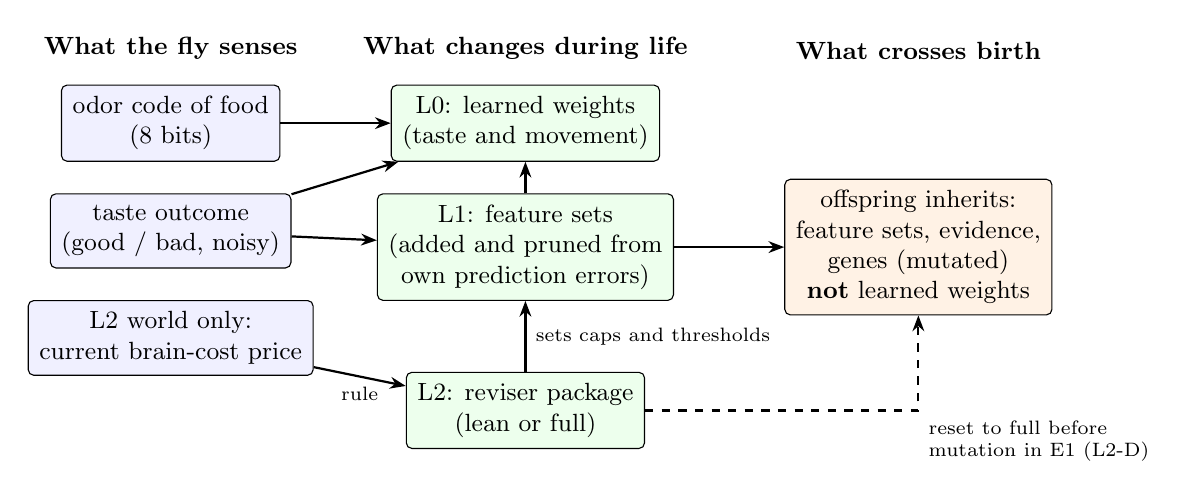
\begin{tikzpicture}[font=\small, node distance=4mm and 6mm,
  box/.style={draw, rounded corners=2pt, align=center, inner sep=4pt, minimum height=9mm},
  sense/.style={box, fill=blue!6}, life/.style={box, fill=green!7}, birth/.style={box, fill=orange!10},
  arr/.style={-{Stealth[length=2mm]}, thick}]
  \node[sense] (odor) {odor code of food\\(8 bits)};
  \node[sense, below=of odor] (taste) {taste outcome\\(good / bad, noisy)};
  \node[sense, below=of taste] (price) {L2 world only:\\current brain-cost price};
  \node[life, right=14mm of odor] (weights) {L0: learned weights\\(taste and movement)};
  \node[life, below=of weights] (masks) {L1: feature sets\\(added and pruned from\\own prediction errors)};
  \node[life, below=9mm of masks] (pkg) {L2: reviser package\\(lean or full)};
  \node[birth, right=14mm of masks] (child) {offspring inherits:\\feature sets, evidence,\\genes (mutated)\\\textbf{not} learned weights};
  \draw[arr] (odor) -- (weights); \draw[arr] (taste) -- (weights); \draw[arr] (taste) -- (masks);
  \draw[arr] (price) -- node[below, font=\scriptsize]{rule} (pkg);
  \draw[arr] (pkg) -- node[right, font=\scriptsize]{sets caps and thresholds} (masks);
  \draw[arr] (masks) -- (weights);
  \draw[arr] (masks) -- (child);
  \draw[arr, dashed] (pkg.east) -| node[below right, font=\scriptsize, align=left]{reset to full before\\mutation in E1 (L2-D)} (child.south);
  \node[above=2mm of odor, font=\bfseries\small] {What the fly senses};
  \node[above=2mm of weights, font=\bfseries\small] {What changes during life};
  \node[font=\bfseries\small] at (child |- weights.north) [anchor=south, yshift=2mm] {What crosses birth};
\end{tikzpicture}
\caption{What a Microverse fly senses, what changes during its life, and what passes to its offspring. In the original L2 experiment the controller's current package was copied to the child and constrained its mutation (dashed arrow); in the controlled re-test (E1) it is reset to the full package first.}
\label{fig:controller}
\end{figure}

\section{Protocol and statistics}
\label{sec:protocol}

\textbf{Prospective specification.} For every confirmatory test, the arms, the outcome, the pass bars and a fresh seed bank were written into a goal document and committed to git before the run. This is an internal discipline, not external pre-registration \citep{nosek2018preregistration}: local commits can be rewritten before they are pushed, and the plans were not lodged with a third party. Design work used practice seeds (101--116 and 301--332). A final ran once on its fresh bank and was never rerun to seek a pass; a redesigned test got a new name and a new bank, and the failed test kept its verdict. Appendix~\ref{app:attempts} lists every attempt.

\textbf{Outcome.} Except for the first goal suite, every test is a paired-solo comparison: each arm lives alone in a world started from the same seed, and the outcome is its \emph{late population}, the mean number of living flies over the 100 snapshots at ticks 10,100 to 20,000, with zero after extinction. Arms that share a seed start identically but do not see identical histories, because behavior changes how the world's random stream is consumed; they are \emph{paired by initial seed}. The first suite (goals G1--G7) used head-to-head competition between two strains and scored the share of the late population; we replaced it after a review showed that a contest with eight seeds is close to a coin flip per seed.

\textbf{Tests.} For each contrast we report the mean paired difference, the number of seeds on which it was positive, a 20,000-resample percentile bootstrap 95\% confidence interval over seeds \citep{efron1993bootstrap}, and a one-sided sign-flip $p$-value. The test's null hypothesis is that each seed's paired difference is equally likely to have either sign (sign symmetry), which holds if the two arm labels are exchangeable within a seed. It is a test against zero, not evidence that an effect exceeds a margin; margins are separate bars on the mean. The $p$-values are exact: the null distribution of the signed sum is enumerated over all $2^n$ sign assignments by dynamic programming on a $0.01$-fly grid. We report values below $10^{-6}$ as $p<10^{-6}$. The runners' own Monte Carlo $p$-values are defective (Section~\ref{sec:verification}); every $p$-value in this paper is recomputed, and where we quote a historical printed value we label it as such.

\textbf{Multiplicity.} We do not correct across tests that asked different questions. Two kinds of multiplicity matter and fresh seeds do not remove either. Across about 20 gated final contrasts, a Bonferroni line of $0.01/20$ would be passed by every headline result but not by P13b-2b ($p \PthirteenTwoBEvorP$). More importantly, worlds and designs were selected on practice seeds: the L2 world was chosen from five candidates for its headroom, and the P13b line tried ten designs. Our positive results therefore show that an effect exists in a world chosen for it, not that it is common.

\section{Results}
\label{sec:results}

Table~\ref{tab:headline} collects the headline fresh-seed results; Figure~\ref{fig:diffs} shows their per-seed differences.

\begin{table}[t]
\centering
\caption{Headline fresh-seed results. Effect is the mean paired difference in late population (flies); exact one-sided sign-flip $p$. All values are generated from committed per-seed data by \texttt{docs/paper/verify.mjs}.}
\label{tab:headline}
\small
\begin{adjustbox}{max width=\textwidth}
\begin{tabular}{@{}llrrrrl@{}}
\toprule
\textbf{Test} & \textbf{Contrast} & \textbf{Seeds ($n$)} & \textbf{Effect} & \textbf{95\% CI} & \textbf{Wins/$n$} & \textbf{$p$} \\
\midrule
G7c & \texttt{SELF} $-$ \texttt{TASTEONLY} & 94001--94096 (96) & \GsevenCTasteMean & \GsevenCTasteCI & \GsevenCTasteWins & $\GsevenCTastePv$ \\
G7c & \texttt{SELF} $-$ \texttt{MOVEONLY} & 94001--94096 (96) & \GsevenCMoveMean & \GsevenCMoveCI & \GsevenCMoveWins & $\GsevenCMovePv$ \\
\midrule
P11b & $R^* - R_{\mathrm{P12}}$ (gate) & 80001--80048 (48) & \PelevenBMean & \PelevenBCI & \PelevenBWins & $\PelevenBPv$ \\
P11b & $R^* - R_0$ (reported) & 80001--80048 (48) & \PelevenBvsRzeroMean & \PelevenBvsRzeroCI & \PelevenBvsRzeroWins & $\PelevenBvsRzeroPv$ \\
\midrule
L2 & \texttt{META} $-$ \texttt{EVO-R} & 95001--95048 (48) & \LtwoEvorMean & \LtwoEvorCI & \LtwoEvorWins & $\LtwoEvorPv$ \\
L2 & \texttt{META} $-$ \texttt{SHAM} & 95001--95048 (48) & \LtwoShamMean & \LtwoShamCI & \LtwoShamWins & $\LtwoShamPv$ \\
L2 & \texttt{META} $-$ \texttt{FIXED} & 95001--95048 (48) & \LtwoFixedMean & \LtwoFixedCI & \LtwoFixedWins & $\LtwoFixedPv$ \\
\bottomrule
\end{tabular}
\end{adjustbox}
\end{table}

\begin{figure}[t]
\centering
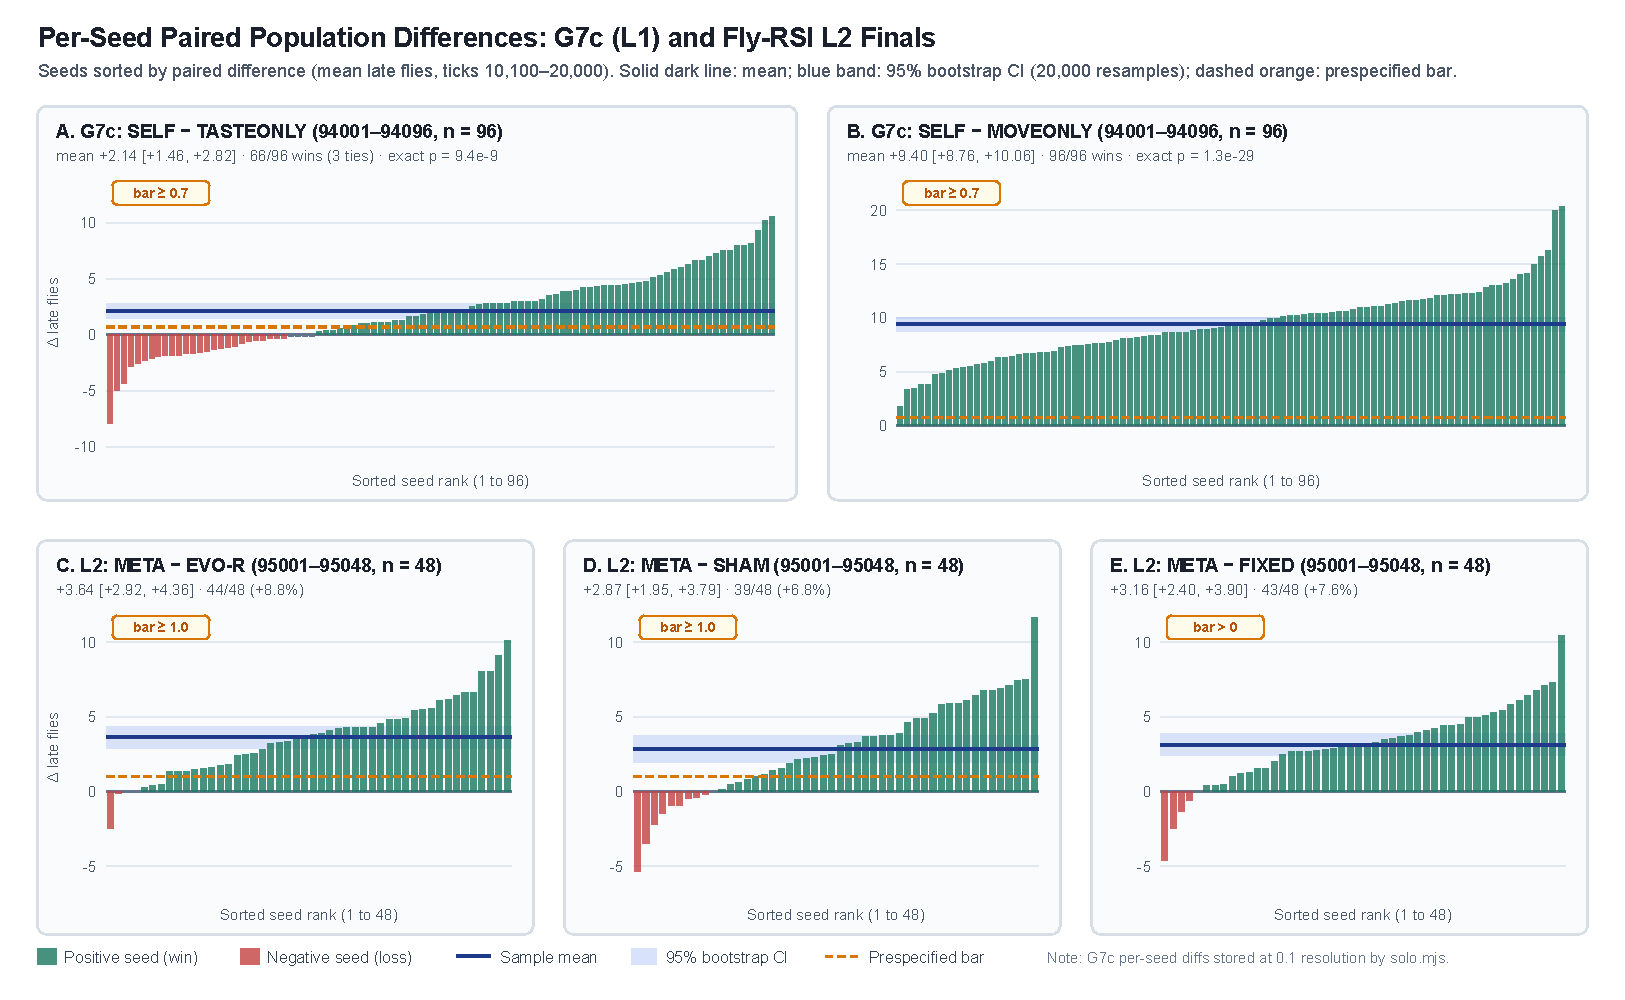
\includegraphics[width=\textwidth]{figures/fig2_g7c_l2_diffs}
\caption{Per-seed paired differences in late population for the G7c final ($n=96$, A--B) and the L2 final ($n=48$, C--E), sorted. Lines show the mean, bands the bootstrap 95\% CI, dashed lines the prespecified bars.}
\label{fig:diffs}
\end{figure}

\subsection{Lifetime learning and feature revision (L0, L1)}

The first world went extinct on every practice seed; nine logged attempts made it livable (Appendix~\ref{app:attempts}). The goal suite G1--G6 then passed two fresh competition finals (seeds 50001--50008 and 60001--60008; Table~\ref{tab:g1-g6}). Lifetime learning beat a frozen brain on 8/8 seeds in both (G4, L0), and self-revising flies beat fixed flies and a random-revision sham on 8/8 (G5, L1). These are eight-seed competition results on the fly as it was before the G7c change; a check against mutation-only evolution was run on practice seeds only.

The next goal asked whether revising movement adds to revising taste (G7). It failed twice in competition (3/8 and 5/8 wins), and its paired-solo successor G7b missed narrowly ($+0.88$ flies, 30/48; printed $p=0.0119$, exact $p \GsevenBP$). A third, separately named test, G7c, allowed a redesign of the movement reviser on practice seeds: an added movement sense now starts at weight 2 with the sign of its evidence, instead of at zero. On 96 fresh seeds, flies revising both systems sustained \GsevenCTasteMean{} more flies than taste-only revision (CI \GsevenCTasteCI) and \GsevenCMoveMean{} more than movement-only revision.

G7c compares the whole movement-revision package against its absence. It does not show that choosing senses from evidence matters, as opposed to switching on a useful sense at a large weight: on practice seeds, simply giving the fly the ``toward best food'' and ``stay'' senses at weight 1 added about 2.9 flies. Experiment E2 tests this directly.

\textbf{E2: does evidence-driven selection matter?} After two blind reviews we ran four controls on the current fly, on 96 fresh seeds under a plan committed before the run (Table~\ref{tab:e1e2}). \texttt{SELF} beat full random revision (\texttt{SHAM}, \EtwoShamMean{} flies) and no revision (\texttt{FIXED}, \EtwoFixedMean), and beat a fly whose taste revision uses evidence but whose movement revision is random (\texttt{MOVESHAM}, \EtwoMoveshamMean{} flies, $p \EtwoMoveshamP$). So choosing movement senses from evidence beats choosing them at random. But a fly with no movement revision that is simply born with the ``toward best food'' and ``stay'' senses at weight 2 (\texttt{GIFT}) did slightly better than \texttt{SELF}: \texttt{SELF} $-$ \texttt{GIFT} $=$ \EtwoGiftMean{} flies (CI \EtwoGiftCI), failing the prespecified gate. The movement half of G7c is therefore matched by a designer who supplies the right senses; what evidence-driven revision adds is finding them without being told, which in this world is worth less than knowing them from birth.

\subsection{An external search over the reviser (P11b)}

P11b asked whether a hand-written hill climber, scored in the world, could improve the taste reviser's five settings. From the designer's tuned reviser $R_0$ there was too little headroom to test, so the search was restarted from $R_{\mathrm{P12}}$, the reviser as it was before forgetting and pruning were added by hand, over a grid that contained those settings. The climber accepted three steps that restored pruning, faster revision and forgetting. On 48 fresh seeds the found reviser $R^*$ beat $R_{\mathrm{P12}}$ by \PelevenBMean{} flies (\PelevenBWins). The gate therefore measures undoing a known handicap, not finding something new. Against $R_0$ the result was \PelevenBvsRzeroMean{} flies (CI \PelevenBvsRzeroCI): not significantly worse, but not shown equal. With the current fly (after G7c), $R_0$ is better by 1.52 flies, and $R^*$ is ahead on only 12 of 48 seeds. P11b is an external search, not in-life self-improvement, and we report it as a positive control for the search machinery.

\subsection{In-life control of the reviser (L2)}

The L2 world was built so that the best reviser package changes during a fly's life. The energy cost of each brain feature switches between $\times 1$ and $\times 12$ of its base cost, independently for each fly, with a mean dwell of 1,000 ticks against a maximum lifespan of 1,200. The state is not inherited. The controller (\texttt{META}) is hand-written: each tick it reads the fly's current price multiplier from the simulator, before any energy is spent, and applies a lean package while the price is high and a full package otherwise. The lean package caps the taste and movement feature sets at the founder sets, prunes hard and blocks new features; in effect, it sheds and stops adding features while they are expensive. Both packages were taken from the headroom analysis.

On 48 fresh seeds \texttt{META} beat evolution of the same two packages (\texttt{EVO-R}: the package flips at birth with probability 0.1) by \LtwoEvorMean{} flies, the same rule driven by an independent fake price (\texttt{SHAM}) by \LtwoShamMean, and the always-full package (\texttt{FIXED}) by \LtwoFixedMean, on a baseline of about 41 flies (7--9\%). The result replicated on new seeds (Section~\ref{sec:verification}).

Much of this is true by construction, and both reviewers said so. Evolution cannot track a non-heritable state that changes within a lifetime, so \texttt{EVO-R} can only be a static mixture. The cue is the simulator's own state, not an estimate the fly forms. The original final also left four questions open, which a controlled re-test (E1) addresses: whether reading the price once at birth gives the same benefit as tracking it; whether the gain runs through revision or is simple feature shedding (no \texttt{METAOFF} or always-lean arm was run); whether the controller acted through offspring mutation as well, since a child copied its parent's current package before mutation; and whether \texttt{SHAM}'s fake price, drawn from the fly's own random stream, perturbed it.

\textbf{E1: decomposing the L2 effect.} The controlled re-test (Table~\ref{tab:e1e2}) ran eight arms on 48 fresh seeds. Every arm re-applies its package each tick, so mutated thresholds are reset alike; a controller's package is reset to the full one before its offspring mutate; and the sham's fake price has its own random stream. All prespecified gates passed. \texttt{META} beat a fly that reads the true price once, at birth, and keeps that package for life (\texttt{BIRTH}, \EoneBirthMean{} flies, $p \EoneBirthP$), so following changes during life adds to choosing well at birth. Birth assignment alone, however, gave \EoneBirthFixedMean{} of \texttt{META}'s \EoneFixedMean{} over the always-full package: about 60\% of the benefit is choosing the right package once. About \EoneSwitchedMeta{} of \texttt{META} flies saw a price switch before they died. \texttt{META} also beat evolution of the packages (\EoneEvorMean), the own-stream sham (\EoneShamMean) and an always-lean fly (\EoneLeanMean). With revision switched off, \texttt{META} and \texttt{NOREV} were identical on every seed, so once the package is reset before birth the controller acts only through L1 revision. That revision is mostly shedding: \texttt{META} carried \EoneFeatMeta{} active features on average against \EoneFeatFixed{} for the always-full fly. Shedding as such does not help (always-lean lost \EoneLeanFixedMean{} flies to always-full); shedding while features are expensive does. The L2 result is best described as a population benefit of state-conditioned package assignment, about two-fifths of which comes from tracking changes during life.

\begin{table}[t]
\centering
\caption{Controls added after blind review (fresh seeds, run once; plan committed before the run). E1: L2 world, $n=48$; E2: default world, $n=96$. Exact one-sided $p$.}
\label{tab:e1e2}
\small
\begin{adjustbox}{max width=\textwidth}
\begin{tabular}{@{}llrrrrl@{}}
\toprule
\textbf{Exp.} & \textbf{Contrast} & \textbf{Effect} & \textbf{95\% CI} & \textbf{Wins/$n$} & \textbf{$p$} & \textbf{Bar} \\
\midrule
E1 & \texttt{META} $-$ \texttt{BIRTH} & \EoneBirthMean & \EoneBirthCI & \EoneBirthWins & $\EoneBirthPv$ & $> 0$: pass \\
E1 & \texttt{META} $-$ \texttt{EVO-R} & \EoneEvorMean & \EoneEvorCI & \EoneEvorWins & $\EoneEvorPv$ & $\ge 1.0$: pass \\
E1 & \texttt{META} $-$ \texttt{SHAM} (own stream) & \EoneShamMean & \EoneShamCI & \EoneShamWins & $\EoneShamPv$ & $\ge 1.0$: pass \\
E1 & \texttt{META} $-$ \texttt{FIXED} & \EoneFixedMean & \EoneFixedCI & \EoneFixedWins & $\EoneFixedPv$ & $> 0$: pass \\
E1 & \texttt{META} $-$ \texttt{LEAN} & \EoneLeanMean & \EoneLeanCI & \EoneLeanWins & $\EoneLeanPv$ & $> 0$: pass \\
E1 & \texttt{BIRTH} $-$ \texttt{FIXED} & \EoneBirthFixedMean & \EoneBirthFixedCI & \EoneBirthFixedWins & $\EoneBirthFixedPv$ & reported \\
E1 & \texttt{METAOFF} $-$ \texttt{NOREV} & \EoneMetaoffMean & \EoneMetaoffCI & \EoneMetaoffWins & & reported \\
\midrule
E2 & \texttt{SELF} $-$ \texttt{SHAM} & \EtwoShamMean & \EtwoShamCI & \EtwoShamWins & $\EtwoShamPv$ & $\ge 0.7$: pass \\
E2 & \texttt{SELF} $-$ \texttt{MOVESHAM} & \EtwoMoveshamMean & \EtwoMoveshamCI & \EtwoMoveshamWins & $\EtwoMoveshamPv$ & $\ge 0.7$: pass \\
E2 & \texttt{SELF} $-$ \texttt{GIFT} & \EtwoGiftMean & \EtwoGiftCI & \EtwoGiftWins & $\EtwoGiftPv$ & $> 0$: \textbf{fail} \\
E2 & \texttt{SELF} $-$ \texttt{FIXED} & \EtwoFixedMean & \EtwoFixedCI & \EtwoFixedWins & $\EtwoFixedPv$ & $\ge 0.7$: pass \\
\bottomrule
\end{tabular}
\end{adjustbox}
\end{table}

\subsection{Compounding (L3) was not reached}
\label{sec:l3}

L3 asks whether L2 control makes L1 revision pay at least $1.5\times$ more than L1 without it. Eight designs and screens were tried; none qualified for a fresh-seed final, and the five reserved final banks are untouched. Table~\ref{tab:l3-hyp} groups them by the hypothesis each one tests; Appendix~\ref{app:l3} gives every number.

\begin{table}[t]
\centering
\caption{The eight L3 designs and screens, grouped by what each tests. None advanced to a final.}
\label{tab:l3-hyp}
\small
\begin{adjustbox}{max width=\textwidth}
\begin{tabular}{@{}p{3.2cm}p{4.6cm}p{6.6cm}@{}}
\toprule
\textbf{Screens} & \textbf{Hypothesis tested} & \textbf{What the result supports} \\
\midrule
L3, L3b (10 practice attempts) & The L2 controller in the L2 world, with harsher or softer prices, amplifies L1 & Best ratio $1.44\times$. Harsher prices raised the ordinary L1 gain as well, so the ratio fell. Not shown for this controller. \\
L3c, L3-I screen 1 & Parking features while expensive amplifies L1 & An apparent $1.78\times$ was partly L1 repairing damage the controller did to inheritance (Section~\ref{sec:controls}). With inheritance fixed, the factorial effect was \LthreeIfactMean{} (CI \LthreeIfactCI). Not shown. \\
L3-I screen 2 & A price on rewriting features at capacity gives a lever & The targeted situation occurred too rarely (0 of 16 worlds qualified) to test anything. Uninformative about compounding. \\
L3-II & Routing structural evidence by a noisy body cue beats a cue-blind scheduler & The oracle beat every static allocation, but a cue-blind scheduler closed about 40\% of its gain; the margin over it ($+1.37$) missed the bar of 2.0. \\
L3-III & The cue-blind scheduler itself compounds L1 & Clearly not: surplus $d=-5.81$ flies, positive on 1 of 16 worlds. \\
L3-IV-H0 & A four-bank world gives an oracle controller enough headroom & The oracle reached $1.58\times$ at toxin 0.60 but its surplus over the $1.5\times$ line was $+0.49$ (CI spans 0), against a required $+4$. Headroom too small to justify a controller. \\
\bottomrule
\end{tabular}
\end{adjustbox}
\end{table}

These are stopping decisions under prespecified bars, not evidence of a ceiling. In the four-bank screen the oracle itself exceeded $1.5\times$; what failed was the margin the protocol demanded before building a controller. Only L3-III gives a clearly negative estimate for the controller it tested. An unregistered four-seed diagnosis suggests where the oracle's expected gain went, chiefly the cost of carrying sixteen founder features that cannot be pruned (Appendix~\ref{app:l3}); we treat it as a hypothesis. We did not demonstrate an L2 lever with enough headroom for $1.5\times$ compounding, and we did not show that none exists.

\section{Controls that changed the answer}
\label{sec:controls}

The most transferable findings are the controls that reversed or narrowed an apparent result.

\textbf{Inheritance damage posing as compounding.} In L3c, parking features while they were expensive raised the L1 payoff ratio to $1.78\times$. A controller-only arm with L1 switched off (\texttt{METAOFF}) then lost 5.15 flies to the no-revision baseline, because offspring born while features were parked did not inherit them; part of the apparent amplification was L1 repairing damage the controller caused. With inheritance repaired, the controller's direct effect became positive (\LthreeImetaoffMean{} flies, $p \LthreeImetaoffP$) and the factorial effect vanished. A factorial design with a controller-only arm should be standard whenever a controller can affect fitness by a route other than the mechanism under test.

\textbf{A coin flip matched an evidence rule.} In the P13b line, an in-life trial-and-revert rule for the reviser's settings beat evolution of those settings (P13b-2b, \PthirteenTwoBEvorMean{} flies, $p \PthirteenTwoBEvorP$), yet a sham that kept or reverted each trial by coin flip did just as well (\PthirteenTwoBShamMean, $p \PthirteenTwoBShamP$). Faster variation plus selection, not the fly's evidence, produced the gain. Beating an evolutionary baseline is not enough to show that an organism used its own evidence. Of ten P13b designs, the only one that passed every gate (A3) tunes a feeding threshold rather than the reviser, and we keep it out of the ladder (Table~\ref{tab:related-rungs}).

\textbf{Controls from blind review.} Two reviewers given only an earlier draft asked for the birth-only, always-lean, controller-only, own-stream-sham and gift controls of experiments E1 and E2. Two of them changed the conclusions. Reading the price once at birth gives most of the L2 benefit (E1), so the claim that the fly ``tracks'' its world rests on the remaining two-fifths. Giving the fly the right movement senses from birth matches evidence-driven movement revision (E2), so G7c shows that revision can find useful senses, not that it finds them better than a designer would. Both results replaced stronger claims in the earlier draft.

\section{Verification}
\label{sec:verification}

The verification plan was committed before its runs (\texttt{docs/PAPER\_VERIFICATION\_PLAN.md}), as was the plan for E1 and E2 (\texttt{docs/PAPER\_REVISION\_PLAN.md}); results are logged in \texttt{docs/PAPER\_VERIFICATION\_LOG.md}.

\textbf{Numbers from raw data.} \texttt{docs/paper/verify.mjs} recomputes every effect, win count, confidence interval and $p$-value from committed per-seed data, checks each against the original logs, and writes the macros this manuscript uses; the figures use the same code. A self-check guards the test: six differences of $+1$ and 42 zeros must give $p=1/64$.

\textbf{Deterministic reruns.} The simulator is deterministic. Rerun at their recorded commits on their own seeds, the G1--G6 finals (both), G7b, G7c, P11b and L2 reproduced exactly; these reruns supplied per-seed data where only summaries had been saved. The P13b finals were not rerun. P11b does not reproduce with current code, because G7c later changed the default fly. A deterministic rerun confirms that the archived numbers match the code, not that the design is sound.

\textbf{Replication on new seeds.} A separate agent ran the G7c and L2 finals once, verbatim, on new banks (6100001--6100048, 6200001--6200096) under unchanged bars. This is a new-seed replication with the same implementation, not an independent reimplementation. Both passed every gate, with effects at least as large as the originals (Table~\ref{tab:replication}).

\begin{table}[t]
\centering
\caption{Replication on new seed banks with the same implementation, run once. Original final values in brackets.}
\label{tab:replication}
\small
\begin{adjustbox}{max width=\textwidth}
\begin{tabular}{@{}llrrrrl@{}}
\toprule
\textbf{Test} & \textbf{Contrast} & \textbf{Effect} & \textbf{95\% CI} & \textbf{Wins/$n$} & \textbf{$p$} & \textbf{Bar} \\
\midrule
L2 & \texttt{META} $-$ \texttt{EVO-R} & \RepLtwoEvorMean{} [\LtwoEvorMean] & \RepLtwoEvorCI & \RepLtwoEvorWins & $\RepLtwoEvorPv$ & $\ge 1.0$: pass \\
L2 & \texttt{META} $-$ \texttt{SHAM} & \RepLtwoShamMean{} [\LtwoShamMean] & \RepLtwoShamCI & \RepLtwoShamWins & $\RepLtwoShamPv$ & $\ge 1.0$: pass \\
L2 & \texttt{META} $-$ \texttt{FIXED} & \RepLtwoFixedMean{} [\LtwoFixedMean] & \RepLtwoFixedCI & \RepLtwoFixedWins & $\RepLtwoFixedPv$ & $> 0$: pass \\
G7c & \texttt{SELF} $-$ \texttt{TASTEONLY} & \RepGsevenCTasteMean{} [\GsevenCTasteMean] & \RepGsevenCTasteCI & \RepGsevenCTasteWins & $\RepGsevenCTastePv$ & $\ge 0.7$: pass \\
G7c & \texttt{SELF} $-$ \texttt{MOVEONLY} & \RepGsevenCMoveMean{} [\GsevenCMoveMean] & \RepGsevenCMoveCI & \RepGsevenCMoveWins & $\RepGsevenCMovePv$ & $\ge 0.7$: pass \\
\bottomrule
\end{tabular}
\end{adjustbox}
\end{table}

\textbf{Sensitivity.} On practice seeds we varied the L2 price contrast ($\times 8$, $\times 16$) and switching rate ($.0005$, $.002$), and the G7c rule-epoch length (2,000 and 4,500 ticks). Every gated contrast stayed positive (Table~\ref{tab:sensitivity}), but on 16 seeds that is a weak requirement and the effect sizes moved: at a $\times 8$ price the L2 advantage over \texttt{EVO-R} and \texttt{SHAM} fell to about one fly and would not clear the original bars. The chosen world sits near the best value tried, as expected for a world selected for headroom.

\begin{table}[t]
\centering
\caption{Sensitivity to world settings (practice seeds 101--116, $n=16$; mean difference, wins, exact $p$). Report-only.}
\label{tab:sensitivity}
\small
\begin{adjustbox}{max width=\textwidth}
\begin{tabular}{@{}llrrr@{}}
\toprule
\textbf{Test} & \textbf{Variant} & \textbf{vs.\ \texttt{EVO-R} / \texttt{TASTEONLY}} & \textbf{vs.\ \texttt{SHAM} / \texttt{MOVEONLY}} & \textbf{vs.\ \texttt{FIXED}} \\
\midrule
L2 & base (price $\times 12$, switch $.001$) & $+3.02$, 14/16, $6\times 10^{-5}$ & $+3.88$, 16/16, $2\times 10^{-5}$ & $+3.05$, 15/16, $2\times 10^{-4}$ \\
L2 & low price ($\times 8$) & $+0.85$, 10/16, $.085$ & $+1.20$, 10/16, $.091$ & $+1.46$, 13/16, $.008$ \\
L2 & high price ($\times 16$) & $+1.19$, 13/16, $.033$ & $+3.27$, 13/16, $.002$ & $+2.50$, 14/16, $2\times 10^{-4}$ \\
L2 & slow switching ($.0005$) & $+3.44$, 14/16, $2\times 10^{-4}$ & $+4.21$, 14/16, $1\times 10^{-4}$ & $+3.80$, 14/16, $9\times 10^{-5}$ \\
L2 & fast switching ($.002$) & $+2.61$, 13/16, $.001$ & $+1.74$, 11/16, $.025$ & $+3.36$, 15/16, $3\times 10^{-5}$ \\
\midrule
G7c & base (epoch 3,000 ticks) & $+2.17$, 15/16, $5\times 10^{-5}$ & $+9.13$, 16/16, $2\times 10^{-5}$ & \\
G7c & short epochs (2,000) & $+2.77$, 12/16, $.006$ & $+9.38$, 16/16, $2\times 10^{-5}$ & \\
G7c & long epochs (4,500) & $+3.05$, 12/16, $.007$ & $+5.88$, 15/16, $1\times 10^{-4}$ & \\
\bottomrule
\end{tabular}
\end{adjustbox}
\end{table}

\textbf{Audit and code defects.} A model given only the code and the claims audited the controls (\texttt{docs/paper/AUDIT\_CONTROLS.md}). It found no information leak (no arm can see the hidden rule or future draws), equal feature rent across arms, and an identical outcome computation in every runner. It also found the L2 issues that E1 addresses. Separately, both Monte Carlo generators in our runners were defective. The original one multiplied a 32-bit linear congruential state in floating point, lost low bits and fell into a cycle of 419 states, giving about 570 distinct sign vectors in 200,000 draws at $n=48$; on a case with exact $p=1/64$ it printed $0.0096$. Its replacement was integer-exact but took its sign from bit 16 of a power-of-two generator, whose period is $2^{17}$: 8,192 distinct sign vectors at $n=48$. Rechecked exactly, no historical pass or fail changes; the closest calls are G7b (printed $0.0119$, exact $\GsevenBPv$, a miss) and P13b-3a (printed $0.0191$, exact $\PthirteenThreeAPv$, a miss).

\section{Related work}
\label{sec:related}

\textbf{Learning, plasticity and evolution.} When learning beats fixed behavior depends on how predictable the environment is within and across generations \citep{stephens1991change,dunlap2009components,dunlap2016reliability}; plasticity theory makes the same point for phenotypes in general \citep{westeberhard2003developmental}. The Baldwin effect describes how learning shapes the evolutionary landscape \citep{baldwin1896new,hinton1987learning}, and evolved plastic networks learn during life under evolved rules \citep{soltoggio2008evolutionary,soltoggio2018born,fernando2018meta,najarro2020meta}. The L2 result is a case of this prediction: in-life control of learning settings beats genetic adaptation when the best setting changes within a lifetime on a cue evolution cannot anticipate. What this paper adds is not the prediction but a breeding-world protocol that separates it from its confounds.

\textbf{Adapting learning settings.} Adapting learning rates and other meta-parameters online is long established, from incremental delta-bar-delta \citep{sutton1992adapting} and gain adaptation \citep{schraudolph1999local} to neuromodulation as meta-parameter control \citep{doya2002metalearning}. Differentiable plasticity and gradient-based meta-learning learn such rules offline \citep{miconi2018differentiable,miconi2020backpropamine,finn2017model,hospedales2022meta}; learned optimizers do so at scale, with mixed returns over tuned baselines \citep{metz2022velo,rezk2023scaling}. Our P13b and L3 results echo the last point: a well-tuned fixed reviser leaves little room for tuning it.

\textbf{Self-improving systems.} G\"odel machines rewrite themselves on proof of improvement \citep{schmidhuber2007godel}; PowerPlay invents tasks and solvers together \citep{schmidhuber2013powerplay}; the Darwin G\"odel Machine evolves coding agents against benchmarks \citep{zhang2025darwin}; statistical certification replaces proof with error-controlled tests \citep{wu2025sgm}. Microverse tests the idea in a closed ecology where improvement must pay off in survival.

\textbf{Artificial-life ecologies.} Microverse belongs with Avida and PolyWorld \citep{ofria2004avida,yaeger1994polyworld}. Work on open-endedness argues that sustained innovation needs a changing environment \citep{bedau2000open,taylor2015requirements,wang2019poet,clune2019aigas,faldor2024omni}, and varying goals can drive structure \citep{kashtan2005spontaneous}; our single hand-built ecology does not test those claims.

\textbf{Earlier work in this project.} Microverse followed a compact-fly line (P5--P16) in an offline surrogate and a many-odor world without breeding. There, a search that invented its own edit operator improved the embodied fly's energy on unseen rules, an embodied replication of its level-2 step failed, and lineages revised their own taste program across generations without a surrogate. Microverse was built to test such claims inside one continuous breeding world with selection.

\section{Limitations}
\label{sec:limitations}

\begin{enumerate}
  \item \textbf{One hand-built world.} All operators, menus, climbers and controllers are hand-written, and the L2 and P13b worlds were chosen for headroom. The results show existence in these worlds, not generality.
  \item \textbf{L2 is a designed switch.} The controller reads the true price and chooses between two preset packages; nothing in the fly discovers the packages or the cue. About 60\% of its benefit is obtained by reading the price once at birth.
  \item \textbf{Movement revision is matched by a gift.} Evidence-driven movement revision beats random revision but not a fly born with the two useful senses; we did not test a gift of other senses or a gift with revision added.
  \item \textbf{Same implementation throughout.} Reruns and the replication use the same code; an independent reimplementation would test the model itself.
  \item \textbf{Internal registration.} Plans were committed to git, not registered externally.
  \item \textbf{Mixed fly versions.} G1--G6 used the fly before G7c changed it; under current code those goals passed on practice seeds only, and P11b's comparison with the designer's reviser reverses.
  \item \textbf{Archival gaps.} G7c stored differences rounded to $0.1$ flies; the G7b and P11b per-seed rows were recovered by rerun.
\end{enumerate}

\section{AI-assistance disclosure}
\label{sec:ai-disclosure}

The human author set the research goals, approved changes in scope and made continuation and stopping decisions, and is responsible for every claim. Much of the work was done with AI models, credited here; they are not listed as authors because they cannot take responsibility for the work.
\begin{itemize}
  \item \textbf{Claude Opus 5.5 (Anthropic)} wrote the Microverse simulator and runners, ran the experiments, kept the goal and result logs, and for this paper planned and ran the verification and the E1/E2 experiments, wrote the exact-test verifier, and revised the manuscript.
  \item \textbf{Claude Fable 5.2 (Anthropic)} audited the earlier experiment line and the first Microverse goals; its review led to withdrawn claims and to the paired-solo design.
  \item \textbf{GPT-6.2 Astra (OpenAI)} gave adversarial advice and wrote the registration wording for the L3 screens, audited the controls for this paper, and reviewed a draft blind; \textbf{GPT-6 Astra} ran the new-seed replication.
  \item \textbf{Gemini 4 Neon (Google)} proposed the four-bank screen, ran its unregistered diagnosis, and wrote the first draft of this paper.
\end{itemize}
Every simulation result was produced by the committed code; no model edited results.

\section{Reproducibility}
\label{sec:repro}

Code, plans, logs and per-seed data are in the \texttt{fly-ecosystem} repository; the simulator and scripts need only Node.js. \texttt{node docs/paper/verify.mjs} regenerates every number in this paper from the data without running a simulation, and \texttt{docs/REPRODUCE\_MICROVERSE.md} gives the command and commit for each final. Spent and reserved seed banks are listed in \texttt{docs/SPENT\_BANKS\_RSI.md}; new work should not reuse them.

\bibliographystyle{plainnat}
\bibliography{refs}

\appendix
% Moved from the v1 main text. Model details for Appendix A.
\section{Microverse model details}
\label{app:model}
\subsection{Ecology and Life Cycle}

Each world runs for $T = 20{,}000$ ticks on a $40\times 40$ toroidal grid with carrying capacity $400$ flies (Table~\ref{tab:world-params}). Eight circular food patches (radius 4, plant density 0.6) hold plants that regrow by $0.08$ units per tick up to capacity $4.0$. Every 50 ticks, one patch chosen uniformly at random is erased and re-seeded at a new random center, forcing flies to relocate rather than camp indefinitely on a single patch.

Each simulation begins with 60 founders placed uniformly at random with initial energy $50$ (30 per strain in two-strain competitions; 60 in solo worlds). On each tick, living flies act in a reproducibly shuffled order: each fly chooses one of 5 moves (stay or step north, east, south, west), pays basal metabolism ($0.06$), movement cost ($0.02$ if stepping), and per-feature brain maintenance cost ($0.0005$ per active taste or movement mask per tick). If a plant with amount $> 0.2$ occupies the destination cell, the fly predicts whether the food is edible; if its predicted probability exceeds \texttt{acceptAt} ($0.4$) or with taste-exploration probability \texttt{tasteEps} ($0.05$), it takes a bite of $\min(\text{amount}, 1.5)$. Good food adds $+\text{take}$ energy; toxic food subtracts $\text{toxin}\times\text{take}$ (default $\text{toxin}=0.6$). Energy is capped at $100$. When a fly's energy reaches \texttt{birthEnergy} ($60$) and total population is below $400$, it pays $30$ energy to spawn an asexual child in an adjacent cell with $25$ energy (the $5$-unit difference is dissipated). Flies die upon energy $\le 0$ (starvation) or age $\ge 1{,}200$ ticks.

\begin{table}[t]
\centering
\caption{Default Microverse ecological parameters and genetic defaults (\texttt{microverse/sim.mjs}, \texttt{microverse/config.mjs}). Values reflect the post-G7c default world (fingerprint \texttt{bdaca307\dots}).}
\label{tab:world-params}
\small
\begin{adjustbox}{max width=\textwidth}
\begin{tabular}{@{}llll@{}}
\toprule
\textbf{Ecology parameter} & \textbf{Default} & \textbf{Brain / gene parameter} & \textbf{Default} \\
\midrule
Grid size (torus) & $40 \times 40$ & Initial taste masks (\texttt{S0Masks}) & 9 (bias + 8 singletons) \\
Run length / snapshot interval & 20,000 / 100 ticks & \texttt{tasteStep} / \texttt{tasteCap} & $4.0$ / $16$ \\
Food patches / radius / density & 8 / 4 / 0.6 & \texttt{tasteZ} / \texttt{tasteEvery} & $3.0$ / $8$ tastings \\
Patch relocation / plant cap / regrow & 50 ticks / 4.0 / 0.08 & \texttt{tasteMemory} / \texttt{tastePrune} & $200$ / $2.0$ \\
Bite size / default toxin & 1.5 / 0.6 & \texttt{acceptAt} / \texttt{tasteEps} & $0.4$ / $0.05$ \\
Basal metabolism / move / brain cost & 0.06 / 0.02 / 0.0005 & Initial move masks (\texttt{MOVE0}) & 6 innate features \\
Founders / capacity / max age & 60 / 400 / 1,200 & \texttt{moveStep} / \texttt{moveCap} / \texttt{eps} & $0.05$ / $12$ / $0.08$ \\
Birth energy / cost / child energy & 60 / 30 / 25 & \texttt{moveZ} / \texttt{moveEvery} / \texttt{movePrune} & $3.0$ / $32$ / $0.5$ \\
Odor kinds / redraw / rule epoch & 16 / 100 / 3,000 ticks & \texttt{moveAddInit} (G7c) / mutation & $2.0$ / $0.1$ \\
Taste label noise / sense radius & 0.05 / 4 cells & Replay reservoir size / replays per bite & 32 / 1 \\
\bottomrule
\end{tabular}
\end{adjustbox}
\end{table}

\subsection{Non-Stationary Walsh-Basis Chemistry}

Each plant belongs to one of $K=16$ odor kinds, each assigned an 8-bit odor code $x \in \{-1,+1\}^8$. Hidden food valence is governed by a Walsh-basis rule over $x$, where for bitmask $m \in \{0,\dots,255\}$ the Walsh feature is $\psi_m(x) = \prod_{b:\, (m \gg b)\,\&\,1} x_b$. Rules cycle deterministically every 3,000 ticks through four families (\texttt{microverse/config.mjs}):
\begin{itemize}
  \item \texttt{pairs}: three disjoint 2-bit Walsh products (weight 1 each, bias 0);
  \item \texttt{staircase}: nested 1-, 2-, 3-, and 4-bit Walsh products on a 4-bit permutation (weights $1,2,2,1$, bias $0.5$);
  \item \texttt{triples}: two disjoint 3-bit products (weight 1) plus one 1-bit term (weight $0.5$, bias 0);
  \item \texttt{single}: one 1-bit Walsh term (weight 1, bias 0).
\end{itemize}
Each rule draws a fresh bit permutation and overall sign $s \in \{-1,+1\}$, with valence $v(x) = s \cdot \operatorname{sign}\!\big(\text{bias} + \sum_j c_j \psi_{m_j}(x)\big)$. Every 100 ticks, the 16 odor codes are redrawn from $\{0,\dots,255\}$ under balanced chemistry: exactly 8 good and 8 bad kinds per draw. Redrawing odor codes prevents flies from memorizing static kind IDs while keeping the hidden rule invariant within each 3,000-tick epoch. When a fly eats a plant, its binary taste label is flipped with probability $0.05$.

\subsection{Dual Brain Architecture: L0 Learning and L1 Self-Revision}

Each fly has two subsystems: a taste predictor and a movement controller. Both separate acquired weights (L0, reset at birth) from heritable structural feature masks and accumulated structural evidence (L1, inherited with optional mutation).

\textbf{Taste subsystem.} A fly holds a list of Walsh masks $M_{\text{taste}}$ (starting from the bias mask $0$ and all 8 singletons, so 9 masks; maximum \texttt{tasteCap} $=16$) with weights $w_i \in [-8,8]$. The model probability is
\[
  p_{\text{model}}(x) = \sigma\!\left(\ln 3 + \frac{1}{\sqrt{|M_{\text{taste}}|}} \sum_{i} w_i \psi_{m_i}(x)\right),
\]
where $\sigma(z) = (1+e^{-z})^{-1}$. A confidence gate compares an exponential moving average (rate $0.05$) of the model's pre-update binary log-loss against the loss of a running base-rate predictor; if the model loss is not strictly lower, the fly falls back to its running base rate, and final output is clipped to $[0.05, 0.95]$ via $0.05 + 0.9\,p$. On each tasting, the fly updates $w$ by one logistic gradient step (\texttt{tasteStep} $=4$) on the current bite and one step on a sample drawn uniformly from a 32-slot reservoir buffer.

For L1 taste self-revision (\texttt{tasteRevise = 'evid'}), the fly maintains decayed correlation evidence $\text{ev}[k]$ over all 256 masks and decayed squared residual $s^2$, updating on every bite with decay $D = 1 - 1/\texttt{tasteMemory}$ and pre-update residual $r$: $\text{ev}[k] \leftarrow D\,\text{ev}[k] + \psi_k(x)\,r$ and $s^2 \leftarrow D\,s^2 + r^2$. Every \texttt{tasteEvery} ($8$) tastings, if $|M_{\text{taste}}| \ge \texttt{tasteCap}$, the fly prunes the weakest higher-order mask ($\operatorname{popcount}(m)>1$) satisfying $|w_i| < \texttt{tastePrune}$ ($2$); founder singletons and bias are never pruned. If a slot is available, the fly forms the candidate set of absent one-bit extensions $m \mid 2^b$ of its current masks, selects $k^* = \arg\max_k |\text{ev}[k]|$, and admits $k^*$ if $|\text{ev}[k^*]| > \texttt{tasteZ}\sqrt{s^2}$ (\texttt{tasteZ} $=3$) at initial weight 0.

\textbf{Movement subsystem.} For each of the 5 candidate moves, the fly computes 6 innate base features (bias, food amount at target cell, expected-value food at target cell, smell within radius 4, local crowding, normalized energy) plus 4 optional senses in the movement sense menu (near smell radius 2, far smell radius 6, indicator for stepping toward the highest-value sensed food cell within radius 4, and indicator for staying on worthwhile edible food). All food-smell features weight food solely by the fly's own expected value $p - (1-p)\cdot\text{toxin}$ for kinds it would accept, with no oracle valence leak. Actions are chosen $\varepsilon$-greedily ($\varepsilon = 0.08$) from a linear value function over movement masks $M_{\text{move}}$ (initialized with innate instinct weights \texttt{MOVE\_INIT}: food $0.5$, EV-food $1.0$, smell $1.0$, crowding $-0.3$). Weights update via an advantage-with-eligibility-trace rule ($\lambda = 0.8$, baseline rate $0.02$, \texttt{moveStep} $=0.05$, reward $\Delta E / 4$). L1 movement revision tracks trace-weighted residual evidence over the menu of optional singletons and move-dependent pairwise feature products, checking every 32 moves, pruning the weakest non-innate feature with $|w| < 0.5$ at cap 12, and admitting the top candidate when $|\text{ev}| > 3\sqrt{s^2}$. In the redesigned G7c operator, an admitted movement sense starts at an evidence-signed weight $\texttt{moveAddInit} \cdot \operatorname{sign}(\text{ev})$ with $\texttt{moveAddInit}=2$ (random sign for the matched sham).

\textbf{Inheritance and opt-in extensions.} At birth, a child inherits its parent's taste masks, movement masks, genes, and structural evidence arrays (never learned weights). Under mutation ($m=0.1$), random mask additions/deletions and multiplicative log-normal gene perturbations ($\exp((u-0.5)\cdot 0.4)$) occur independently. All L2, L3, and P13b world modifications (\texttt{brainSwitch}, \texttt{rewriteCost}, \texttt{attention}, \texttt{quad}, \texttt{toxinNiche}, \texttt{toxinSwitch}, etc.) are strictly opt-in; every extension after G7c verified that the default-world fingerprint (\texttt{bdaca307\dots}) remained bit-for-bit unchanged.


% Moved from the v1 main text. Supporting tables and the detailed L3 narrative for Appendix B.

\section{Supporting tables and the L3 screens in detail}

\label{app:tables}

\begin{table}[t]
\centering
\caption{Fresh-seed final banks and reserved untouched banks in the Microverse program. Practice work used seeds 101--108, 101--116, and 301--332 (plus exploratory 501--504). No fresh bank was ever reused.}
\label{tab:seed-banks}
\small
\begin{adjustbox}{max width=\textwidth}
\begin{tabular}{@{}llllr@{}}
\toprule
\textbf{Bank} & \textbf{Experiment} & \textbf{Status} & \textbf{Raw JSON committed} & \textbf{Seeds} \\
\midrule
50001--50008 & G1--G7 Final Run 1 (\texttt{73ffefe}) & G1--G6 closed; G7 failed & Yes (added for paper) & 8 \\
60001--60008 & G1--G7 Final Run 2 (\texttt{da995b0}) & G1--G6 closed; G7 failed & Yes (added for paper) & 8 \\
70001--70048 & G7b paired solo (\texttt{da995b0}) & Failed ($p=0.0119$) & Yes (exact rerun) & 48 \\
80001--80048 & P11b external L2 search (\texttt{07b54e7}) & Passed ($+5.73$) & Yes (exact rerun) & 48 \\
90001--90048 & P13b parts 1--4 (\texttt{6521edb}) & 1 passed; 2, 3, 4 failed & Yes & 48 \\
91001--91048 & P13b-2b trials vs.\ mutation (\texttt{228d500}) & Passed ($+1.24$) & Yes & 48 \\
92001--92048 & P13b-3a/3b shadow trials (\texttt{e75f8d2}) & Both failed & Yes & 48 \\
93001--93048 & P13b A3 (\texttt{acceptAt}, \texttt{d75ad75}) & Passed (decision gene) & Yes & 48 \\
94001--94096 & G7c redesigned move reviser (\texttt{95a3f21}) & Passed ($+2.14$, $+9.40$) & Yes & 96 \\
95001--95048 & Fly-RSI L2 reviser switch (\texttt{1ef4381}) & Passed ($+3.64$ vs.\ EVO-R) & Yes & 48 \\
\midrule
96001--96048 & L3b (reserved) & Untouched (failed practice) & N/A & (48) \\
97001--97048 & L3c (reserved) & Untouched (stopped att.\ 3) & N/A & (48) \\
763001--763048 & L3-I (reserved) & Untouched (scr.\ 1 \& 2 missed) & N/A & (48) \\
852001--852048 & L3-II (reserved) & Untouched (stage A missed) & N/A & (48) \\
874001--874048 & L3-III (reserved) & Untouched (stage B missed) & N/A & (48) \\
\bottomrule
\end{tabular}
\end{adjustbox}
\end{table}

\begin{table}[t]
\centering
\caption{Microverse core ladder results (G1--G6) across two fresh-seed final runs (8 fresh seeds each; winner-take-all competition shares except G1 and G6 solo runs). Source: \texttt{docs/MICROVERSE\_LOG.md}.}
\label{tab:g1-g6}
\small
\begin{adjustbox}{max width=\textwidth}
\begin{tabular}{@{}lllll@{}}
\toprule
\textbf{Goal} & \textbf{Test} & \textbf{Final Run 1 (50001--50008)} & \textbf{Final Run 2 (60001--60008)} & \textbf{Status} \\
\midrule
G1 & \texttt{FIXED} alone (livability) & Pass ($\ge 7/8$ ok) & Pass (8/8 ok) & Closed \\
G2 & \texttt{ORACLE} vs.\ \texttt{FIXED} & 8/8 wins & 8/8 wins & Closed \\
G3 & \texttt{FIXED} vs.\ \texttt{RANDMOVE} & 8/8 wins & 8/8 wins & Closed (instinct caveat) \\
G4 (L0) & \texttt{FIXED} vs.\ \texttt{FROZEN} & 8/8 wins & 8/8 wins & Closed \\
G5 (L1) & \texttt{SELF} vs.\ \texttt{FIXED} \& \texttt{SHAM} & 8/8 \& 8/8 wins & 8/8 \& 8/8 wins & Closed (8/8 vs.\ \texttt{EVO} on practice only) \\
G6 (L1) & \texttt{SELF} alone (adaptation) & Gain $0.394$, late $0.775$ & Gain $0.362$, late $0.711$ & Closed (rediscovery) \\
\bottomrule
\end{tabular}
\end{adjustbox}
\end{table}

\begin{table}[t]
\centering
\caption{Related rungs, failed tests, split sub-tests, and amended tests on fresh seeds. Exact $p$-values and CIs come from committed per-seed data via \texttt{verify.mjs}; P13b-3a/3b CIs from \texttt{figures/compute\_stats.mjs}. G7 and G7b are logged values. No verdict changes under the exact test.}
\label{tab:related-rungs}
\small
\begin{adjustbox}{max width=\textwidth}
\begin{tabular}{@{}llllrrrl@{}}
\toprule
\textbf{Test} & \textbf{Target / Note} & \textbf{Seeds ($n$)} & \textbf{Contrast} & \textbf{Effect} & \textbf{95\% CI} & \textbf{Wins/$n$} & \textbf{Verdict (exact $p$)} \\
\midrule
G7 (FR1) & Competition move L1 & 50001--08 (8) & \texttt{SELF} vs.\ \texttt{TASTE} & share 0.33 & N/A & 3/8 & \textbf{FAILED} \\
G7 (FR2) & Competition move L1 & 60001--08 (8) & \texttt{SELF} vs.\ \texttt{TASTE} & share 0.625 & N/A & 5/8 & \textbf{FAILED} \\
G7b & Paired solo (\texttt{da995b0}) & 70001--48 (48) & \texttt{SELF}$-$\texttt{TASTE} & \GsevenBMean & \GsevenBCI & \GsevenBWins & \textbf{FAILED} ($\GsevenBPv$; runner $0.0119$) \\
\midrule
P13b-1 & Own tuning vs.\ none & 90001--48 (48) & \texttt{META}$-$\texttt{FIXED} & \PthirteenPartsFixedMean & \PthirteenPartsFixedCI & \PthirteenPartsFixedWins & \textbf{PASSED} ($\PthirteenPartsFixedPv$) \\
P13b-2 & Trials vs.\ mutation & 90001--48 (48) & \texttt{META}$-$\texttt{EVO-R} & \PthirteenPartsEvorMean & \PthirteenPartsEvorCI & \PthirteenPartsEvorWins & \textbf{FAILED} ($\PthirteenPartsEvorPv$) \\
P13b-3 & Evidence vs.\ coin flip & 90001--48 (48) & \texttt{META}$-$\texttt{SHAM} & \PthirteenPartsShamMean & \PthirteenPartsShamCI & \PthirteenPartsShamWins & \textbf{FAILED} ($\PthirteenPartsShamPv$) \\
P13b-2b & Faster trials (\texttt{metaK}=3) & 91001--48 (48) & \texttt{META}$'-$\texttt{EVO-R} & \PthirteenTwoBEvorMean & \PthirteenTwoBEvorCI & \PthirteenTwoBEvorWins & \textbf{PASSED} ($\PthirteenTwoBEvorPv$; vs.\ SHAM \PthirteenTwoBShamMean, $p \PthirteenTwoBShamP$) \\
P13b-3a & Shadow keep accuracy & 92001--48 (48) & bal.\ acc.\ $-0.5$ & $+0.0044$ & $[-0.0002,+0.0090]$ & 27/48 & \textbf{FAILED} ($\PthirteenThreeAPv$; runner printed $0.0191$) \\
P13b-3b & Distance to $R^*$ & 92001--48 (48) & \texttt{SHAM}$-$\texttt{META} & $+0.06$ & $[-0.36,+0.49]$ & 26/48 & \textbf{FAILED} (runner $0.408$) \\
\midrule
P13b A3 & 10th design; \texttt{acceptAt} & 93001--48 (48) & \texttt{META}$-$\texttt{EVO-R} & \PthirteenAthreeEvorMean & \PthirteenAthreeEvorCI & \PthirteenAthreeEvorWins & \textbf{PASSED under A3} ($\PthirteenAthreeEvorPv$) \\
        & (decision threshold, &                & \texttt{META}$-$\texttt{SHAM} & \PthirteenAthreeShamMean & \PthirteenAthreeShamCI & \PthirteenAthreeShamWins & (not reviser tuning; \\
        & not reviser)         &                & \texttt{META}$-$\texttt{FIXED} & \PthirteenAthreeFixedMean & \PthirteenAthreeFixedCI & \PthirteenAthreeFixedWins & constructed \texttt{toxinSwitch}) \\
\bottomrule
\end{tabular}
\end{adjustbox}
\end{table}

\begin{table}[t]
\centering
\caption{Forking-paths audit across the Microverse line (commits \texttt{d459944}--\texttt{16b4372}). Complete per-attempt details are in Appendix~\ref{app:attempts}.}
\label{tab:forking}
\small
\begin{adjustbox}{max width=\textwidth}
\begin{tabular}{@{}lrrrl@{}}
\toprule
\textbf{Goal / Line} & \textbf{Practice att./scr.} & \textbf{Amendments / re-tests} & \textbf{Finals run (fresh seeds)} & \textbf{Final outcome} \\
\midrule
G1--G6 (core ladder) & 12 att.\ (+ checks) & 1 (G6 validity rule) & 2 shared (16) & All 6 closed (FR1 \& FR2) \\
G7 / G7b / G7c & 9 att.\ (+ 4 checks) & 2 (\texttt{G7b}, \texttt{G7c}) & 4 (144 dedicated) & G7 $\times 2$ fail, G7b fail, G7c pass \\
P11b (external L2) & 2 headroom + 24 props & 1 (\texttt{A1}: start $R_{\mathrm{P12}}$) & 1 (48) & Passed (orig.\ P11 stays failed) \\
P13b (related line) & 10 designs, 16 att. & 3 (\texttt{A1}--\texttt{A3}) + 3 splits & 4 (192) & A1 not shown; A3 pass (\texttt{acceptAt}) \\
Fly-RSI L2 & 5 worlds + 1 att. & 0 & 1 (48) & Passed (95001--95048) \\
Fly-RSI L3 & 8 designs, 20 batches & 7 successor regs & 0 (0; 240 reserved) & Not shown (0 finals) \\
\bottomrule
\end{tabular}
\end{adjustbox}
\end{table}

\subsection{The L3 screens in detail}

\label{app:l3}

\begin{table}[t]
\centering
\caption{All eight prespecified L3 compounding designs and headroom screens. None qualified for a fresh-seed final run. Intervals are 95\% bootstrap CIs where raw JSON is committed.}
\label{tab:l3-screens}
\small
\begin{adjustbox}{max width=\textwidth}
\begin{tabular}{@{}llllll@{}}
\toprule
\textbf{\#} & \textbf{Design} & \textbf{Mechanism / World} & \textbf{Bar (Practice / Screen)} & \textbf{Observed Result} & \textbf{Outcome} \\
\midrule
1 & L3 & \texttt{brainSwitch} $\times 1/\times 12$, 5 rule att. & Ratio $\ge 1.5\times$ ($d>0, p<.01$) & Best ratio $1.44\times$ (att.\ 1) & Failed practice \\
2 & L3b & \texttt{brainSwitch} hi $\in\{20,30,50\}$, 5 att. & Ratio $\ge 1.5\times$ + L2 gates & Best ratio $1.444\times$ (att.\ 5) & Failed practice \\
3 & L3c & hi $20$ + dormant parking, 3/5 att. & Ratio $\ge 1.5\times$ + L2 gates & $1.778\times$ ($p=.017$), confound & Stopped att.\ 3 \\
4 & L3-I scr1 & Parking + \texttt{inheritFull} ($n=48$) & $f>0$ ($p<.01$) \& $\ge 33/48$ & $f=-0.45$ $[-4.52,+3.89]$, 19/48 & Missed (1.46$\times$) \\
5 & L3-I scr2 & \texttt{RewriteCost} swap trial ($n=16$) & $\ge 12/16$ ($\ge 20$ chk, $\ge 10\%$) & 0/16 qualify (2 wins / 230 chk) & Missed St.\ A \\
6 & L3-II & 2-bank attention \texttt{bankPairs} ($n=16$) & \texttt{ORAC}$-$\texttt{BLIND} $\ge 2.0$, $\ge 12/16$ & $+1.37$ $[-0.36,+3.16]$, 10/16 & Missed St.\ A \\
7 & L3-III & Evidence-routed \texttt{attentionA} ($n=16$) & $g>0, d>0, \ge 9/16$ $d>0$ & $g=+13.39$, $d=-5.81$, 1/16 & Missed St.\ B \\
8 & L3-IV-H0 & 4-bank \texttt{quadBankPairs} ($n=16\times 2$) & $d_O\ge 4$ ($\ge 13/16$), $b\ge 4$ & .60: $d_O=+0.49$ (8/16), $b=+2.54$ & Missed both \\
  &          &                                          &                                & .85: $d_O=-1.91$ (4/16), $b=+2.62$ & toxins \\
\bottomrule
\end{tabular}
\end{adjustbox}
\end{table}

\subsection{Energy-Cost Switching and Dormant Parking (L3, L3b, L3c, L3-I Screen 1)}

In the L2 \texttt{brainSwitch} world ($\times 1/\times 12$), five practice attempts reached a maximum L1 gain ratio of $1.44\times$ (Attempt 1: $(\text{META}-\text{NOREV})/(\text{FIXED}-\text{NOREV}) = (44.73-32.74)/(41.09-32.74) = 1.44 < 1.5$). Raising the costly-state multiplier to $\times 20, \times 30, \times 50$ in \textbf{L3b} backfired on the ratio: harsher brain costs inflated the ordinary L1 denominator ($\texttt{FIXED}-\texttt{NOREV}$) because \texttt{NOREV} accumulated mutated movement masks it could never prune. Even adding fast shedding and a 300-tick fast-regrowth phase topped out at $1.444\times$.

\textbf{L3c} fixed the multiplier at $\times 20$ and introduced dormant-feature parking (\texttt{park}/\texttt{unpark}): storing added masks and their weights cost-free while brain cost is high and restoring them when cost falls. Parking added masks alone gave $1.453\times$ (20/48 seeds with $d>0$, $p=0.59$). Extending parking to weak founder singletons ($|w|<1$ in Attempt 2, $|w|<2$ in Attempt 3) pushed the headline ratio to $1.746\times$ ($p=0.041$) and $1.778\times$ (34/48, $p=0.017$), at which point the run was deliberately stopped after 3 of 5 attempts because parking founder singletons saves energy even without L1 discovery.

External review by GPT-6.2 Astra exposed two structural flaws in L3c: heavy tails (on Attempt 2, a single seed, 113, where \texttt{FIXED} went extinct gave $d=+59.6$, contributing $+1.24$ of the $+2.51$ mean $d$) and the missing direct-effect control \texttt{METAOFF} (running the controller with L1 disabled). Running the pre-specified descriptive \texttt{METAOFF} diagnostic on L3c Attempt 3 (\texttt{fly-rsi-l3c-metaoff-practice.json}) revealed a surprise: \texttt{METAOFF} averaged $21.75$ vs.\ \texttt{NOREV} $26.90$ ($-5.15$ flies, 4 extinctions), because offspring born while singletons were parked failed to inherit the parked masks and, lacking L1, could never recover them. Part of L3c's apparent factorial gain ($+7.97$) was therefore L1 repairing inheritance damage caused by the controller.

\textbf{L3-I Screen 1} (\texttt{e43bda8}, \texttt{fly-rsi-l3i-screen1-practice.json}) fixed inheritance via \texttt{inheritFull} (children inherit the deduplicated union of active and parked masks, and transient controller packages reset before birth; verified on 431 births with 0 defects), upgraded to Scorer v2, and added a factorial mean gate $f = d - (\texttt{METAOFF}-\texttt{NOREV}) > 0$ plus a typical-world binomial sign gate ($f > 0$ on $\ge 33/48$ seeds, exact binomial $p=0.0066$). With inheritance repaired, \texttt{METAOFF} gained \LthreeImetaoffMean{} flies over \texttt{NOREV} ($30.26$ vs.\ $26.90$, 95\% CI \LthreeImetaoffCI, exact $p \LthreeImetaoffP$). Ordinary L1 gain was $+10.17$ ($\texttt{FIXED}-\texttt{NOREV}$, $[+7.59,+12.57]$), and L1 gain under the controller was $+14.81$ ($\texttt{META}-\texttt{METAOFF}$, $[+13.01,+17.05]$), an observed ratio of $1.456\times$ (logged $1.46\times$). Screen 1 missed all three compounding gates: original $d = \LthreeIdOrigMean$ (\LthreeIdOrigCI, exact $p \LthreeIdOrigP \ge 0.01$; Scorer v2 printed $0.01085$), factorial mean $f = \LthreeIfactMean$ (\LthreeIfactCI, exact $p \LthreeIfactP$), and factorial sign $19/48$ (bar $\ge 33/48$).

\subsection{Rewrite-Price Gating: L3-I Screen 2 (RewriteCost)}

To eliminate direct energy savings in \texttt{METAOFF} by construction, \textbf{L3-I Screen 2} (\texttt{RewriteCost}, registered verbatim by Astra in \texttt{a373341}) replaced \texttt{brainSwitch} with a switching energy fee ($0.15$ vs.\ $3.00$, flip rate $0.002$) charged only when committing a taste-mask swap at full capacity, evaluated by a 16-tasting shadow trial against a hurdle gene \texttt{swapHurdle} $\in \{0, 0.025, 0.075, 0.15, \text{NEVER}\}$. Preflight tickwise lockstep tests passed with zero divergent ticks over 20,000 ticks (ensuring $f = d$ identically). However, Stage A (seeds 101--116, hurdle \texttt{NEVER}; \texttt{fly-rsi-l3i-screen2-stageA.json}) failed decisively: \textbf{0/16} seeds qualified against the bar of $\ge 12/16$ seeds with $\ge 20$ blocked checks and $\ge 10\%$ positive-score rate. Across all 16 worlds there were only 5--36 blocked full-cap checks per seed (230 total), 102 nominations, 80 cancellations due to ordinary live edits occurring during the 16-tasting window, 13 pending at death, 9 completions, and 2 wins total (both on seed 114, 15 checks). The targeted full-cap bottleneck is simply too rare in Microverse, retiring the operator without implying an L1 ceiling.

\subsection{Attention-Limited Structural Routing: L3-II and L3-III}

The next mechanism targeted L1's information bottleneck rather than energy cost. \textbf{L3-II} (\texttt{50e0a25}) introduced an opt-in rule family \texttt{bankPairs} splitting the 8 odor bits into Bank A (bits 0--3) and Bank B (bits 4--7), placing one target pair in each bank. Each fly had a private reliable bank switching at $0.004$/tick; L0 perceived the clean odor normally, while L1's structural evidence could route only one bank (15 masks) per tasting, with bits in the unreliable bank flipped independently with probability $q=0.5$. A noisy bodily cue named the reliable bank with accuracy $0.90$.

In Stage A (seeds 101--116, \texttt{fly-rsi-l3ii-stageA.json}), \texttt{ORACLE} ($58.29$ flies, common-tape loss $0.5654$ nats/bite) beat all five static allocations (\texttt{S0} $50.72$ through \texttt{S100} $51.80$, locked \texttt{FIXED} $=$ \texttt{S50} at $56.00$, loss $0.6712$) by $+2.28$ to $+7.56$ flies ($12/16$ wins vs.\ \texttt{S50}) and $-0.1058$ to $-0.1128$ nats/bite, confirming that structural routing works as a mechanism. Yet a mandatory cue-blind evidence scheduler (\texttt{BLIND}, which routes $80\%$ greedily by an exponentially smoothed bank utility built from prior pair correlations predicting new residuals) reached $56.91$ flies (loss $0.6338$), erasing roughly $40\%$ of \texttt{ORACLE}'s population advantage over \texttt{S50}. \texttt{ORACLE} minus \texttt{BLIND} was $+1.37$ flies ($[-0.36,+3.16]$, $10/16$ wins), missing both Stage A bars ($\ge 2.0$ flies and $\ge 12/16$ wins), so L3-II stopped.

\textbf{L3-III} (\texttt{8af02b7}) promoted the cue-blind scheduler itself to \texttt{META} (writing its decision explicitly to \texttt{genes.attentionA}, tested against an independent sensory-twin \texttt{SHAM}). Stage A (seeds 301--316, \texttt{fly-rsi-l3iii-stageA.json}) re-locked \texttt{FIXED} $=$ \texttt{S75} ($55.88$ flies). Stage B (seeds 317--332, \texttt{fly-rsi-l3iii-stageB.json}) missed sharply: ordinary L1 gain was large ($g = \texttt{S75} - \texttt{NOREV} = +13.39$ flies, $[+11.89,+14.89]$, 16/16), so $1.5\times$ compounding required \texttt{META} to add $+6.70$ flies over \texttt{S75}. Instead, $m = \texttt{META} - \texttt{S75} = +0.88$ ($[-0.14,+1.97]$, 10/16; ratio $1.066\times$), yielding $d = m - 0.5g = -5.81$ ($[-7.32,-4.21]$) with only \textbf{1/16} seeds $d > 0$ (bar $\ge 9/16$). Telemetry showed \texttt{META} barely tracked the true reliable bank (match rate $0.530$ vs.\ $0.500$ for \texttt{S75}), earning its small $+0.88$-fly premium from longer same-bank sampling runs ($4.68$ vs.\ $2.65$ tastings) and balanced admissions ($5{,}196$ A / $5{,}321$ B total across 16 seeds vs.\ $3{,}826$ / $1{,}635$ for \texttt{S75}).

\subsection{Four-Bank Oracle Headroom (L3-IV-H0) and Post-Hoc Diagnosis}

To test whether increasing the bank dilution penalty from 1-of-2 to 1-of-4 could open sufficient headroom, \textbf{L3-IV-H0} (proposed by Gemini 4 Neon, cross-examined and registered by Astra in \texttt{12b8e7f}) expanded odors to 16 bits across four 4-bit banks (\texttt{quadBankPairs}, one true pair per bank, \texttt{tasteCap} $=24$, 39 static allocations, toxins $0.60$ and $0.85$ on seeds 101--116; no final bank reserved).

L3-IV-H0 \textbf{missed at both toxins} :
\begin{itemize}
  \item \textbf{Toxin 0.60:} \texttt{NOREV} $42.40$, best static $F = \texttt{S10} = [0,0.5,0.25,0.25]$ at $48.27$ ($g = +5.87$, $[+4.92,+6.98]$, 16/16), \texttt{BLIND} $49.15$, \texttt{ORACLE} $51.69$, \texttt{TRUE\_ORACLE} $63.19$ ($\alpha = 0.28$). Although \texttt{ORACLE} beat \texttt{S10} by $+3.42$ flies ($[+2.09,+4.69]$, 15/16, ratio $1.58\times$), its compounding surplus was only $d_O = (\texttt{ORACLE}-F)-0.5g = +0.49$ ($[-1.25,+2.02]$, 8/16 vs.\ bars $\ge 4.0$ and $\ge 13/16$), and $\texttt{ORACLE}-\texttt{BLIND} = +2.54$ ($[+1.25,+3.85]$, 13/16 vs.\ bar $\ge 4.0$).
  \item \textbf{Toxin 0.85:} \texttt{NOREV} $31.26$, best static $F = \texttt{S20} = [0.25,0.25,0.25,0.25]$ at $41.74$ ($g = +10.48$, $[+8.35,+12.68]$, 16/16), \texttt{BLIND} $42.45$, \texttt{ORACLE} $45.07$, \texttt{TRUE\_ORACLE} $55.02$ ($\alpha = 0.44$). Here $d_O = -1.91$ ($[-3.75,+0.02]$, 4/16) and $\texttt{ORACLE}-\texttt{BLIND} = +2.62$ ($[+0.87,+4.68]$, 13/16), both missing the $4.0$-fly bar.
\end{itemize}
Telemetry at toxin $0.60$ showed that oracle routing accelerated discovery: \texttt{ORACLE} achieved $1.000$ bank-match accuracy, $1{,}981$ admissions per seed, $637$ correct-pair admissions per seed ($6.2\times$ \texttt{S10}'s $102$ and $3.0\times$ \texttt{BLIND}'s $212$), and $2.28$ true pairs held per newborn (vs.\ $0.99$ in \texttt{S10} and $1.46$ in \texttt{BLIND}). Yet this sixfold jump in correct feature discovery translated into only $+3.42$ flies, leaving an apparent $+11.5$-fly gap below \texttt{TRUE\_ORACLE} ($63.19$).

An exploratory post-hoc diagnosis by Gemini 4 Neon on four fresh non-bank seeds (501--504; unregistered, no confidence intervals) suggests where the expected gain went. These are hypotheses from four seeds, not established mechanisms:
\begin{enumerate}
  \item \textbf{The \texttt{TRUE\_ORACLE} gap is mostly feature count, not rule knowledge.} On seeds 501--504 at toxin $0.60$, \texttt{NOREV} averaged $41.55$, \texttt{S10} $46.77$, \texttt{BLIND} $48.74$, and \texttt{ORACLE} $49.88$. Comparing \texttt{TRUE\_5} (bias plus 4 true pairs $=5$ masks: $62.71$ flies) against \texttt{TRUE\_21} (bias plus 16 unprunable founder singletons plus 4 true pairs $=21$ masks: $53.29$ flies) suggests a cost of about 9.4 flies for carrying 16 founder singletons that cannot be pruned. The split into about 4.2 flies of maintenance energy and 5.3 flies of overfitting comes from one further ablation and has no stated uncertainty. Even god-mode \texttt{TRUE\_21} reached only $d_O \approx +3.9 < 4$.
  \item \textbf{Cap crowding was not supported.} \texttt{ORACLE} sat at its 24-mask cap on only $5\%$ of fly-ticks; raising the cap to 40 ($49.97$), disabling mutation ($47.29$), pruning harder ($49.57$), and raising \texttt{tasteZ} ($46.21$) all failed to help \texttt{ORACLE}.
  \item \textbf{Removing founder singletons fails in the opposite direction.} Starting from bias-only \texttt{[0]} with direct within-bank candidates collapsed \texttt{NOREV} to $16.96$ (and $0$ at toxin $0.85$), inflating $g$ so much that the $1.5\times$ bar demanded more flies than \texttt{TRUE\_5} achieves.
  \item \textbf{Movement L1 compresses taste-routing margins.} In taste-only runs, \texttt{ORACLE} beat \texttt{S10} by $+5.70$ flies; enabling movement L1 added $+3.74$ flies to \texttt{S10} but only $+1.15$ to \texttt{ORACLE}.
\end{enumerate}

These observations are hypotheses about why the oracle surplus was small in the four-bank world. They do not establish a general ceiling: the oracle reached a ratio of $1.58\times$ at toxin $0.60$, above $1.5\times$, and missed only the prespecified margin of $+4$ flies (Section~\ref{sec:l3}).

% Generated by docs/paper/attempts2tex.mjs from docs/paper/attempts.md. Do not edit.
\section{Forking-paths ledger}
\label{app:attempts}
This appendix lists every design loop, amendment, headroom screen, diagnostic and fresh-seed final in the Microverse line (commits \texttt{d459944} to \texttt{16b4372}), so that each pass can be read against the attempts that preceded it. Failed and superseded attempts are kept. Practice seeds were 101--116 and 301--332; fresh banks were each run once. The verification banks of Section~\ref{sec:verification} (6100001--6100048 and 6200001--6200096) were also spent once, after this ledger closed, as were the banks of the revision experiments E1 and E2 (6300001--6300048 and 6400001--6400096).

\subsection{Microverse Core Ladder (G1--G7, G7b, G7c)}
Primary sources: \texttt{docs/\allowbreak{}MICROVERSE\_GOALS.\allowbreak{}md}, \texttt{docs/\allowbreak{}MICROVERSE\_LOG.\allowbreak{}md}.
{\footnotesize\setlength{\tabcolsep}{3pt}\renewcommand{\arraystretch}{1.15}
\begin{longtable}{@{}>{\raggedright\arraybackslash}p{1.75cm}>{\raggedright\arraybackslash}p{2.6cm}>{\raggedright\arraybackslash}p{4.3cm}>{\raggedright\arraybackslash}p{4.75cm}>{\raggedright\arraybackslash}p{2.15cm}@{}}
\toprule
\textbf{Goal} & \textbf{Step (commit)} & \textbf{Change} & \textbf{Outcome} & \textbf{Seeds} \\
\midrule
\endhead
G1--G7 & Baseline (\texttt{d459944}) & Initial sim, strains, universal suite (\texttt{MICROVERSE\_GOALS.\allowbreak{}md} fixed before tuning) & G1--G5, G7 failed (all worlds extinct ticks 570--1015); G6 spurious pass on dying worlds & Practice \texttt{101\textendash{}108} \\
G6 & Validity amendment (\texttt{d459944}) & Added livability clause to G6 before any tuning: world alive at tick 20,000 in $\ge$ 7/8 seeds & Rule updated & --- \\
G1 & Attempt 1 (\texttt{9c34740}) & More food (8 patches, regrow 0.08) & 0/8 ok (extinct ticks 600--1900) & Practice \texttt{101\textendash{}108} \\
G1 & Attempt 2 (\texttt{9c34740}) & Milder toxin (1.5 $\to$ 0.6) & 0/8 ok & Practice \texttt{101\textendash{}108} \\
G1 & Attempt 3 (\texttt{9c34740}) & Movement learning: advantage + eligibility trace replacing TD & 0/8 ok (1 seed reached tick 12,578) & Practice \texttt{101\textendash{}108} \\
G1 & Attempt 4 (\texttt{9c34740}) & Cheaper reproduction (breed at 60, cost 30) & 0/8 ok & Practice \texttt{101\textendash{}108} \\
G1 & Attempt 5 (\texttt{9c34740}) & Lower metabolism (0.06, move 0.02) & 2/8 ok (deaths cluster after rule switches) & Practice \texttt{101\textendash{}108} \\
G1 & Attempt 6 (\texttt{9c34740}) & Bigger world (40$\times$40, 12 patches) & 2/8 ok & Practice \texttt{101\textendash{}108} \\
G1 & Attempt 7 (\texttt{9c34740}) & Taste-exploration gene (5\% taste when predicted bad) & 3/8 ok & Practice \texttt{101\textendash{}108} \\
G1 & Attempt 8 (\texttt{9c34740}) & Expected-value accept threshold gene (0.4) & 2/8 ok (base-rate swings 4--12 of 16 cause famines) & Practice \texttt{101\textendash{}108} \\
G1 & Attempt 9 (\texttt{9c34740}) & Balanced chemistry (exact 8 good / 8 bad odor kinds per draw) & \textbf{Practice PASS (7/8)}; suite passes G1, G3 (7/8, .88), G5 (8/8, 8/8), G6 (.20/.53); fails G2 (5/8, .63), G4 (0/8), G7 (1/8 vs TASTEONLY) & Practice \texttt{101\textendash{}108} \\
G2 / G4 & Decomposition check (\texttt{d3c2e6a}) & Taste-learning-only vs FROZEN (0/8); move-learning-only vs FROZEN (4/8) & Isolated taste learning chasing noise & Practice \texttt{101\textendash{}108} \\
G2 / G4 & Attempt 1 (\texttt{d3c2e6a}) & Confidence gate: trust taste model only while running log-loss < base-rate loss & FIXED vs FROZEN rises 0/8 $\to$ 5/8 & Practice \texttt{101\textendash{}108} \\
G2 / G4 & Attempt 2 (\texttt{d3c2e6a}) & Expected-value smell \& food movement features \texttt{p $-\allowbreak{}$ (1$-\allowbreak{}$p)$\cdot$toxin} (counting only accepted food) & \textbf{Practice PASS G1--G5 (all 8/8)}; G6 fails (.181/.566), G7 fails (5/8 vs TASTEONLY); null control FIXED vs FIXED = 9/24 (.38, 0 extinct) & Practice \texttt{101\textendash{}108} (plus 24 null pairings) \\
G6 & Attempt 1 (\texttt{73ffefe}) & Evidence forgetting (\texttt{tasteMemory = 200}, decay \texttt{1$-\allowbreak{}$1/\allowbreak{}200}) + prune weakest added taste mask with \texttt{$|$w$|$ < 2} (matched in SHAM) & \textbf{Practice PASS G1--G6} (G6 gain .368, late .757); G7 fails (3/8, .47) & Practice \texttt{101\textendash{}108} \\
G7 & Headroom check 1 (\texttt{73ffefe}) & Planner measuring instrument vs TASTEONLY & 5/8 wins (share .72) --- modest room & Practice \texttt{101\textendash{}108} \\
G7 & Attempt 1 (\texttt{73ffefe}) & Movement-revision evidence uses decaying trace & 3/8 (.45) --- no progress & Practice \texttt{101\textendash{}108} \\
G7 & Attempt 2 (\texttt{73ffefe}) & Bug fix: disallow duplicate (\texttt{bias $\times$ x}) and move-invariant movement candidates & 5/8 (.54) & Practice \texttt{101\textendash{}108} \\
G7 & Attempt 3 (\texttt{73ffefe}) & Prune weakest added movement feature (\texttt{$|$w$|$ < 0.\allowbreak{}5}) when full & \textbf{Practice PASS G1--G7} (G7 6/8, .66) & Practice \texttt{101\textendash{}108} \\
\textbf{G1--G7} & \textbf{Final Run 1} (\texttt{73ffefe} (logged \texttt{83c94eb})) & Full universal suite frozen before run & \textbf{G1--G6 CLOSED} (G2--G5 all 8/8; G6 gain .394, late .775); \textbf{G7 FAILED} (SELF vs TASTEONLY 3/8, .33; vs MOVEONLY 8/8) & \textbf{Fresh \texttt{50001\textendash{}50008}} (8 seeds, spent) \\
G7 & Attempt 4 (world) (\texttt{da995b0}) & Faster food relocation (every 50 ticks, 8 patches); planner headroom rises to 8/8 & SELF vs TASTEONLY 2/8 (movement learning helps 6/8 vs instinct-only, revision does not) & Practice \texttt{101\textendash{}108} \\
G7 & Attempt 5 (brain) (\texttt{da995b0}) & Movement sense menu (optional bits 6--9: near smell r2, far smell r6, toward best food, stay) & 3/8 & Practice \texttt{101\textendash{}108} \\
G7 & Diagnostic (\texttt{da995b0}) & Set \texttt{brainCost = 0} & 6/8 (revealed feature cost 0.002 ate the gain) & Practice \texttt{101\textendash{}108} \\
G7 & Attempt 6 (world) (\texttt{da995b0}) & Lower \texttt{brainCost} to 0.0005 (still nonzero) & \textbf{Practice PASS G1--G7} (G7 7/8, .89) & Practice \texttt{101\textendash{}108} \\
\textbf{G1--G7} & \textbf{Final Run 2} (\texttt{da995b0} (logged \texttt{83c94eb})) & Full universal suite re-run because world changed & \textbf{G1--G6 CLOSED} (all 8/8; G6 gain .362, late .711); \textbf{G7 FAILED} (SELF vs TASTEONLY 5/8, .625) & \textbf{Fresh \texttt{60001\textendash{}60008}} (8 seeds, spent) \\
G7 & Attempt 7 (dropped) (\texttt{83c94eb}) & Movement evidence forgetting & 6/8 on \texttt{101\textendash{}108}, 10/16 on \texttt{301\textendash{}316} --- dropped, not adopted & Practice \texttt{101\textendash{}108}, \texttt{301\textendash{}316} \\
G7 & World check (dropped) (\texttt{83c94eb}) & Bigger world (56$\times$56, 16 patches) & 7/16 --- confounded (relocation rate halved per patch), dropped & Practice \texttt{101\textendash{}116} (16 seeds) \\
G1--G6 & Validity checks (\texttt{83c94eb}) & Fable review audit at \texttt{da995b0}: order swaps (0/8), SELF vs EVO (8/8), G3 instinct caveat (8/8), FROZEN eating check, G6 rediscovery check, arm parity, label-leak audit & Confirmed G1--G6 validity; Fable verdict on G7 = "not shown" (pooled 18/32 vs null 18/40) & Practice \texttt{101\textendash{}108} \\
\textbf{G7b} & \textbf{Separately named re-test (frozen)} (\texttt{83c94eb} $\to$ \texttt{beee842}) & Paired solo late population (\texttt{solo.\allowbreak{}mjs}) on unchanged code \texttt{da995b0}; practice estimate (\texttt{101\textendash{}116}): +1.41 (13/16, p = .033); one-shot bar: $\ge$ 0.7 flies \& p < .01 & \textbf{FAILED} on SELF $-$ TASTEONLY: +0.88 (30/48, printed p = .0119; exact p = .0130 after rerun); SELF $-$ MOVEONLY +7.81 (48/48, p < .00001). G7b stays failed. & Practice \texttt{101\textendash{}116}; \textbf{Fresh \texttt{70001\textendash{}70048}} (48 seeds, spent) \\
G7c & Re-test frozen + headroom (\texttt{9563c68} $\to$ \texttt{dd0ea19}) & Allow redesign of movement reviser ($\le$ 5 practice attempts on 48 seeds); 96 fresh seeds. Baseline +.86 (31/48, p=.033). Headroom (\texttt{101\textendash{}116}): planner +5.24 (16/16); giving toward+stay at w=1 adds +2.92 (13/16) & Headroom confirmed; diagnosed slow weight ramp from 0 & Practice \texttt{101\textendash{}116}, \texttt{301\textendash{}332} \\
G7c & Attempt 1 (\texttt{dd0ea19}) & Evidence-signed start weight \texttt{moveAddInit = 1} for added movement senses (random sign in SHAM) & +2.39 vs TASTEONLY (36/48, p < .00001) & Practice \texttt{101\textendash{}116}, \texttt{301\textendash{}332} \\
G7c & Attempt 2 (adopted) (\texttt{dd0ea19}) & \texttt{moveAddInit = 2} (applied to SELF, SHAM, MOVEONLY; fingerprint changes to \texttt{bdaca307\dots{}}) & \textbf{+2.47 vs TASTEONLY} (42/48, p < .00001); +9.46 vs MOVEONLY (48/48); universal suite practice \texttt{101\textendash{}108} (\texttt{suite-\allowbreak{}dev-\allowbreak{}1795046397911.\allowbreak{}json}) passes G1--G7 (all 8/8, G6 gain .422) & Practice \texttt{101\textendash{}116}, \texttt{301\textendash{}332} \\
\textbf{G7c} & \textbf{Final Run} (\texttt{95a3f21}) & Paired solo on 96 fresh seeds (bar $\ge$ 0.7 \& p < .01 both contrasts) & \textbf{PASSED}: SELF $-$ TASTEONLY +2.14 (66/96, p < .00001), SELF $-$ MOVEONLY +9.40 (96/96, p < .00001). Pooled G7b+G7c = +1.72 (mixes code versions). & \textbf{Fresh \texttt{94001\textendash{}94096}} (96 seeds, spent) \\
\bottomrule
\end{longtable}}

\subsection{Microverse Level-2 External Search (P11b) and Related In-Lineage Tuning Line (P13b)}
Primary sources: \texttt{docs/\allowbreak{}MICROVERSE\_L2\_GOALS.\allowbreak{}md}, \texttt{docs/\allowbreak{}MICROVERSE\_L2\_LOG.\allowbreak{}md}. Note: Original P11 and P13 from the earlier compact-fly line stay \textbf{FAILED}.
{\footnotesize\setlength{\tabcolsep}{3pt}\renewcommand{\arraystretch}{1.15}
\begin{longtable}{@{}>{\raggedright\arraybackslash}p{1.75cm}>{\raggedright\arraybackslash}p{2.6cm}>{\raggedright\arraybackslash}p{4.3cm}>{\raggedright\arraybackslash}p{4.75cm}>{\raggedright\arraybackslash}p{2.15cm}@{}}
\toprule
\textbf{Goal} & \textbf{Step (commit)} & \textbf{Change} & \textbf{Outcome} & \textbf{Seeds} \\
\midrule
\endhead
P11b & Initial headroom H1 (from \texttt{R0}) (\texttt{d60c3ea} $\to$ \texttt{e36cdca}) & Single-knob grid perturbations around hand-tuned \texttt{R0} (bar $\ge$ 1.5 flies) & \textbf{BLOCKED (H1 failed)}: best change \texttt{z = 1.\allowbreak{}5} gave +1.05 < 1.5; \texttt{R0} already hand-tuned in G6 & Practice \texttt{101\textendash{}116} \\
P11b & Amendment A1 + headroom H1$'$ (\texttt{e36cdca}) & Reset start point to pre-tuning \texttt{R\_P12} (\texttt{tasteMemory = 1e12}, \texttt{tastePrune = 0}); H1$'$ check \texttt{R0 $-\allowbreak{}$ R\_P12} & H1$'$ passed: +6.4 flies (16/16, p = .00002) & Practice \texttt{101\textendash{}116} \\
P11b & Climber search (\texttt{9688222} $\to$ \texttt{ec3047c}) & Hand-written 1-step climber (\texttt{l2search.\allowbreak{}mjs}, seed 4242, 24 proposals, accept $\ge$ +0.5) & Accepted 3 steps (\texttt{tastePrune 0$\to$.\allowbreak{}5} +2.15; \texttt{tasteEvery 8$\to$4} +.85; \texttt{tasteMemory 1e12$\to$800} +3.13); 21 rejected $\to$ \texttt{R*} (train 55.91 vs \texttt{R0} 56.17) & Practice \texttt{101\textendash{}116} \\
\textbf{P11b} & \textbf{Final Run} (\texttt{07b54e7}) & Gate \texttt{R* $-\allowbreak{}$ R\_P12 $\ge$ 1.\allowbreak{}0}, p < .01; reported \texttt{R* $-\allowbreak{}$ R0} & \textbf{PASSED}: \texttt{R* $-\allowbreak{}$ R\_P12} = +5.73 (48/48, p < .00001); \texttt{R* $-\allowbreak{}$ R0} = $-$0.54 (21/48, p = .89, n.s.) & \textbf{Fresh \texttt{80001\textendash{}80048}} (48 seeds, spent) \\
P13b & Design 1: H2 (from \texttt{R0}) (\texttt{d60c3ea} $\to$ \texttt{e36cdca}) & Per-family oracle schedule over \texttt{R} in normal world (bar $\ge$ 1.5) & \textbf{BLOCKED (H2 failed)}: oracle < 1 fly over best fixed & Practice \texttt{101\textendash{}116} \\
P13b & Design 1 (A1): 4 practice attempts + H3 (\texttt{e36cdca} $\to$ \texttt{4fefc6b}) & Start at \texttt{R\_P12}: Att 1 direction rules (vs EVO-R +.13, SHAM $-$.51); Att 2 drop lengthen ($-$.56, +.44); Att 3 trial-and-revert running loss (+1.49, +.26, +6.36 vs FIXED); Att 4 window means (+.85, $-$.38); H3 switch-timed oracle (+.03/$-$.65/$-$.57) & \textbf{BLOCKED}: no rule beats SHAM by $\ge$ 1.0; H3 shows no headroom in normal world & Practice \texttt{101\textendash{}116} \\
P13b & Design 2: H3 fast switching (\texttt{4fefc6b}) & Rule switches every 600 ticks; oracle (50/800) vs fixed memory 200 & \textbf{BLOCKED}: oracle +2.47 vs fixed +1.81 $\to$ oracle $-$ best fixed $\approx$ +0.66 < 1.0 & Practice \texttt{101\textendash{}116} \\
P13b & Designs 3--4: H4 volatility world (\texttt{051b771}) & Calm 4,000t / burst 2,000t (every 150t); Variant A (noise .05), Variant B (noise .15) & \textbf{BLOCKED}: Var A oracle $-$ best fixed $\approx$ +1.1 (< 1.5 headroom bar); Var B $\approx$ 0 & Practice \texttt{101\textendash{}116} \\
P13b & Design 5: H5 long lives (\texttt{02b3026}) & Volatility Variant A with \texttt{maxAge = 6000} & \textbf{BLOCKED}: oracle +1.79 vs fixed +1.40 $\to$ gap $\approx$ +0.39 < 1.5 & Practice \texttt{101\textendash{}116} \\
P13b & Design 6: H6 individual sensor noise (\texttt{f90d8b5}) & Non-heritable per-fly \texttt{noiseNiche} [.02, .3]; learning-rate oracle & \textbf{BLOCKED}: best per-fly oracle $-$ best fixed step = $-$0.33 & Practice \texttt{101\textendash{}116} \\
P13b & Design 7: H7 habitats (\texttt{957d446}) & Left half calm, right half volatile (every 150t); habitat oracle & \textbf{BLOCKED}: best habitat oracle $-$ \texttt{R*} = $-$0.47 & Practice \texttt{101\textendash{}116} \\
P13b & Design 8: Amendment A2 (\texttt{acceptAt}, H8 + 4 attempts + diag) (\texttt{6f6b2a9} $\to$ \texttt{b300032}) & Non-heritable \texttt{toxinNiche} [.2, 3]; extended R = \texttt{acceptAt} (decision threshold, not reviser). H8 oracle +8.36 (16/16). 4 practice attempts (trial, EV, 2$\times$ risk-averse EV, prior+EV) + 32-seed diag & \textbf{BLOCKED}: best vs SHAM +.37 (att 2); diag (\texttt{301\textendash{}332}) showed ORACLE +2.21 vs SHAM is pre-evidence protection only; post-evidence META +.02 vs SHAM & Practice \texttt{101\textendash{}116}, \texttt{301\textendash{}332} \\
P13b & Design 9: H9 dual food (\texttt{26efe96}) & \texttt{dualFood}: fruit stable vs leaf switching every 150t; diet oracle & \textbf{BLOCKED}: best diet oracle $-$ best fixed ($\infty$) = $-$0.35 & Practice \texttt{101\textendash{}116} \\
\textbf{P13b-1..4} & \textbf{Split parts Final (A1 att 3)} (\texttt{e7d9619} $\to$ \texttt{6521edb}) & Single final scoring P13b-1 (vs FIXED), -2 (vs EVO-R), -3 (vs SHAM), -4 (full P13b) & \textbf{P13b-1 PASSED} (+5.96, 46/48, p < .00001); \textbf{P13b-2 FAILED} (+.53, 29/48, p = .131); \textbf{P13b-3 FAILED} ($-$.02, 26/48, p = .516); \textbf{P13b-4 FAILED} & \textbf{Fresh \texttt{90001\textendash{}90048}} (48 seeds, spent) \\
\textbf{P13b-2b} & \textbf{Re-test trials vs mutation} (\texttt{fbe4087} $\to$ \texttt{228d500}) & 3 practice attempts on 48 seeds (\texttt{metaK} $\in$ \{3, 12, 2\}; \texttt{metaK=3} selected at +1.73 vs ref \texttt{metaK=6} +1.90) $\to$ fresh final & \textbf{PASSED}: META$'$ $-$ EVO-R = +1.24 (34/48, exact p = .0024); reported vs SHAM +.25 (p = .28, n.s.), vs FIXED +5.80 (47/48) & Practice \texttt{101\textendash{}116}, \texttt{301\textendash{}332}; \textbf{Fresh \texttt{91001\textendash{}91048}} (48 seeds, spent) \\
P13b-3 & Headroom check (perfect keep) (\texttt{9888c49}) & \texttt{trialoracle} (keeps iff step moves toward \texttt{R*}) vs coin-flip SHAM (\texttt{metaK=3}, 48 seeds) & \textbf{BLOCKED}: ORACLE $-$ SHAM = $-$0.42 (21/48, p = .83) & Practice \texttt{101\textendash{}116}, \texttt{301\textendash{}332} \\
\textbf{P13b-3a/3b} & \textbf{Shadow-trial split Final} (\texttt{e455fc1} $\to$ \texttt{7de7117} $\to$ \texttt{e75f8d2}) & 4 shadow-trial practice attempts (\texttt{metaK} $\in$ \{6 [sham bug], 24, 48, 16\}; \texttt{metaK=16} selected at 3a .5076 p=.0048, 3b +.37 p=.026) $\to$ fresh final & \textbf{P13b-3a FAILED} (.5044, 27/48, printed p = .0191, exact p = .033 > .01); \textbf{P13b-3b FAILED} (SHAM$-$META dist +.06, p = .408) & Practice \texttt{101\textendash{}116}, \texttt{301\textendash{}332}; \textbf{Fresh \texttt{92001\textendash{}92048}} (48 seeds, spent) \\
\textbf{P13b (A3)} & \textbf{Design 10: Amendment A3 (\texttt{acceptAt})} (\texttt{ab573b7} $\to$ \texttt{aff0f0a} $\to$ \texttt{d75ad75}) & In-life switching toxin sensitivity (\texttt{toxinSwitch = .\allowbreak{}005}); H10 oracle +10.71 vs fake +.27; Att 1 tracks felt damage to \texttt{.\allowbreak{}2/\allowbreak{}.\allowbreak{}75} (practice +9.29 vs EVO-R, +10.15 vs SHAM, 48/48) $\to$ fresh final & \textbf{PASSED under A3}: +9.48 vs EVO-R, +8.86 vs SHAM, +9.12 vs FIXED (all 48/48, p < .00001). Labelled: tunes decision threshold \texttt{acceptAt}, not reviser; 10th design. & Practice \texttt{101\textendash{}116}, \texttt{301\textendash{}332}; \textbf{Fresh \texttt{93001\textendash{}93048}} (48 seeds, spent) \\
\bottomrule
\end{longtable}}

\subsection{Bounded Fly-RSI Ladder: L2 and L3 (All 8 L3 Designs / Screens)}
Primary sources: \texttt{docs/\allowbreak{}FLY\_RSI\_GOALS.\allowbreak{}md}, \texttt{docs/\allowbreak{}FLY\_RSI\_LOG.\allowbreak{}md}.
{\footnotesize\setlength{\tabcolsep}{3pt}\renewcommand{\arraystretch}{1.15}
\begin{longtable}{@{}>{\raggedright\arraybackslash}p{1.75cm}>{\raggedright\arraybackslash}p{2.6cm}>{\raggedright\arraybackslash}p{4.3cm}>{\raggedright\arraybackslash}p{4.75cm}>{\raggedright\arraybackslash}p{2.15cm}@{}}
\toprule
\textbf{Goal} & \textbf{Step (commit)} & \textbf{Change} & \textbf{Outcome} & \textbf{Seeds} \\
\midrule
\endhead
Pre-L2 & 5 headroom worlds (\texttt{5272589}) & (1) \texttt{senseDrift} sign flips (oracle +.77); (2) \texttt{senseDrift} permutation ($-$.54); (3) \texttt{brainSwitch} $\times$1/$\times$12 sw .004 (oracle +3.69, fake +1.78); (4) $\times$1/$\times$20 sw .002 (+2.98, fake +.44); (5) $\times$1/$\times$12 sw .001 (\textbf{+3.05, 15/16; fake $-$.83}) & World (5) chosen and frozen (prior perception bug in sense-drift caught by fingerprint and discarded) & Practice \texttt{101\textendash{}116} \\
\textbf{L2} & Practice Att 1 $\to$ \textbf{Final Run} (\texttt{5272589} $\to$ \texttt{a8e5e6b} $\to$ \texttt{1ef4381}) & \texttt{brainTrack} switches L1 taste/move reviser genes between lean \& full packages from a perfect, noise-free reading of the current brain-cost multiplier. Practice Att 1: +3.12 vs EVO-R, +3.55 vs SHAM, +3.64 vs FIXED (all $\ge$ 41/48). Final run once (NOREV omitted because L3 failed practice). & \textbf{L2 PASSED}: META 44.83, SHAM 41.96, EVO-R 41.19, FIXED 41.67; META $-$ EVO-R +3.64 (44/48), META $-$ SHAM +2.87 (39/48), META $-$ FIXED +3.16 (43/48); exact p $\le$ 1.5e-7; replicated on new seeds 6100001--6100048. & Practice \texttt{101\textendash{}116}, \texttt{301\textendash{}332}; \textbf{Fresh \texttt{95001\textendash{}95048}} (48 seeds, spent) \\
\textbf{L3 (Design 1)} & Practice Attempts 1--5 (\texttt{5272589} $\to$ \texttt{a8e5e6b}) & \texttt{brainSwitch} $\times$1/$\times$12 sw .001; bar L1 ratio $\ge$ 1.5$\times$. Att 1 lean while costly (1.44$\times$); Att 2 lean taste only (1.18$\times$); Att 3 lean move only (1.18$\times$); Att 4 +300t fast regrowth (1.38$\times$); Att 5 keep strong prune 2/1 (1.39$\times$) & \textbf{FAILED practice} (best 1.44 < 1.5); \textbf{no final run} & Practice \texttt{101\textendash{}116}, \texttt{301\textendash{}332} \\
\textbf{L3b (Design 2)} & Practice Attempts 1--5 (\texttt{2c898e9} $\to$ \texttt{0fd4ab1}) & \texttt{brainSwitch} hi $\in$ \{20, 30, 50\} + rule form; reserved bank \texttt{96001\textendash{}96048}. Att 1 hi 20 (1.372$\times$); Att 2 hi 50 (1.026$\times$); Att 3 hi 30 (1.106$\times$); Att 4 hi 20 + lean fast shed (1.395$\times$); Att 5 +300t fast regrowth (1.444$\times$) & \textbf{FAILED practice} (best 1.444 < 1.5); \textbf{no final run}; bank \texttt{96001\textendash{}96048} untouched & Practice \texttt{101\textendash{}116}, \texttt{301\textendash{}332} \\
\textbf{L3c (Design 3)} & Practice Attempts 1--3 + META-OFF diagnostic (\texttt{0fd4ab1} $\to$ \texttt{e1fe9c5} $\to$ \texttt{3450a39}) & Fixed hi 20 + dormant feature parking (\texttt{park}/\texttt{unpark}); reserved bank \texttt{97001\textendash{}97048}. Att 1 park added (1.453$\times$, 20/48, p=.59); Att 2 +park singles $|$w$|$<1 (1.746$\times$, 30/48, p=.041; seed 113 heavy tail); Att 3 +park singles $|$w$|$<2 (1.778$\times$, 34/48, p=.017) & \textbf{STOPPED after Att 3} (slots 4--5 unused; bank \texttt{97001\textendash{}97048} untouched). Descriptive META-OFF diag (\texttt{fly-\allowbreak{}rsi-\allowbreak{}l3c-\allowbreak{}metaoff-\allowbreak{}practice.\allowbreak{}json}): META-OFF 21.75 vs NOREV 26.90 ($-$5.15, 4 extinctions) revealed inheritance-loss confound; Astra also flagged float-LCG scorer bug & Practice \texttt{101\textendash{}116}, \texttt{301\textendash{}332} \\
\textbf{L3-I Scr 1 (Design 4)} & Parking + Inheritance Law (\texttt{e43bda8} $\to$ \texttt{a373341}) & L3c Att 3 + \texttt{inheritFull} (repertoire deduplicated, controller package reset before birth) + Scorer v2 + factorial mean/sign gates ($\ge$ 33/48); reserved bank \texttt{763001\textendash{}763048} & \textbf{MISSED} (\texttt{fly-\allowbreak{}rsi-\allowbreak{}l3i-\allowbreak{}screen1-\allowbreak{}practice.\allowbreak{}json}): direct METAOFF$-$NOREV = +3.36 (exact p = .0057); L1 gain 14.81 vs 10.17 (1.456$\times$); original d = +2.92 (exact p = .012); factorial f = $-$0.45 (exact p = .58, 19/48 vs bar 33/48) & Practice \texttt{101\textendash{}116}, \texttt{301\textendash{}332} \\
\textbf{L3-I Scr 2 (Design 5)} & RewriteCost Stage A (\texttt{a373341} $\to$ \texttt{4ea16c8} $\to$ \texttt{0369464}) & Replace \texttt{brainSwitch} with \texttt{rewriteCost} (0.15 / 3.00, sw .002) + 16-tasting shadow swap trial (\texttt{swapHurdle}). Locksteps passed (0 divergent ticks/20,000). Stage A bar: $\ge$ 12/16 seeds with $\ge$ 20 checks \& $\ge$ 10\% win rate & \textbf{MISSED at Stage A} (\texttt{fly-\allowbreak{}rsi-\allowbreak{}l3i-\allowbreak{}screen2-\allowbreak{}stageA.\allowbreak{}json}): \textbf{0/16 qualify} (5--36 blocked checks/seed; 230 checks, 102 nominations, 80 cancellations, 13 pending-at-death, 9 completions, 2 wins total on seed 114). Bank \texttt{763001\textendash{}763048} untouched & Practice \texttt{101\textendash{}116} \\
\textbf{L3-II (Design 6)} & Attention-limited structural revision Stage A (\texttt{50e0a25} $\to$ \texttt{ada5b25} $\to$ \texttt{1493dc6} $\to$ \texttt{34f84b4}) & Two 4-bit odor banks (\texttt{bankPairs}), 1 routed bank/tasting, unreliable bank bit-flip q=.5, private receptor sw .004, .90 cue; reserved bank \texttt{852001\textendash{}852048}. Integrity passed. Stage A bar: ORACLE beats all 5 statics \& BLIND by $\ge$ .01 nats \& $\ge$ 2.0 flies, $\ge$ 12/16 wins vs FIXED \& BLIND & \textbf{MISSED at Stage A} (\texttt{fly-\allowbreak{}rsi-\allowbreak{}l3ii-\allowbreak{}stageA.\allowbreak{}json}): ORACLE (58.29, .5654) beat all statics (+2.28..+7.56 flies, $-$.1058..$-$.1128 nats, 12/16 vs locked S50 56.00), but missed vs BLIND (56.91, .6338): +1.37 flies (bar 2.0), 10/16 wins (bar 12). Bank \texttt{852001\textendash{}852048} untouched & Practice \texttt{101\textendash{}116} \\
\textbf{L3-III (Design 7)} & Evidence-routed attention Stages A \& B (\texttt{8af02b7} $\to$ \texttt{69971d1} $\to$ \texttt{3a0aa03} $\to$ \texttt{1e91a4f}) & \texttt{L3II\_WORLD}; META = former BLIND writing \texttt{attentionA} (no bodily cue); SHAM = independent sensory twin; reserved bank \texttt{874001\textendash{}874048}. Integrity passed. Stage A (\texttt{301\textendash{}316}) re-locked FIXED = S75 (55.88). Stage B (\texttt{317\textendash{}332}) bar: mean g > 0, mean d > 0, $\ge$ 9/16 d > 0 & \textbf{MISSED at Stage B} (\texttt{fly-\allowbreak{}rsi-\allowbreak{}l3iii-\allowbreak{}stageB.\allowbreak{}json}): g = +13.39, META $-$ S75 = +0.88, d = $-$5.81, \textbf{1/16} seeds d > 0 (bar 9). Telemetry: META match rate .530 vs S75 .500; route run 4.68 vs 2.65. Bank \texttt{874001\textendash{}874048} untouched & Practice \texttt{301\textendash{}316} (St A), \texttt{317\textendash{}332} (St B) \\
\textbf{L3-IV-H0 (Design 8)} & Four-bank routing headroom screen (\texttt{12b8e7f} $\to$ \texttt{bcc991d} $\to$ \texttt{d67b3d4}) & 16-bit odor, 4 banks (\texttt{quadBankPairs}), tasteCap 24, 39 static allocations, ORACLE/BLIND/TRUE\_ORACLE at toxins .60 \& .85; reserves no final bank. Integrity passed. Bars: mean g $\ge$ 3, dO $\ge$ 4 ($\ge$ 13/16), ORACLE$-$BLIND $\ge$ 4 ($\ge$ 12/16) & \textbf{MISSED at both toxins} (\texttt{fly-\allowbreak{}rsi-\allowbreak{}l3iv-\allowbreak{}h0.\allowbreak{}json}): toxin .60 $\to$ g = +5.87, dO = +0.49 (8/16), ORACLE$-$BLIND = +2.54 (13/16), $\alpha$ = .28; toxin .85 $\to$ g = +10.48, dO = $-$1.91 (4/16), ORACLE$-$BLIND = +2.62 (13/16), $\alpha$ = .44. L3-IV stops before any controller & Practice \texttt{101\textendash{}116} \\
L3-IV-H0 (post-hoc) & Exploratory diagnosis (unregistered) (\texttt{16b4372}) & Gemini 4 Neon read-only ablations on 4 new seeds (TRUE\_21 vs TRUE\_5, cap=40, mutation off, stronger pruning, higher Z, taste-only vs +move L1, zero-singleton \texttt{[0]}) & Identified 9.4-fly tax from 16 unprunable founder singletons (\~{}4.2 energy + \~{}5.3 L0 overfit), concave saturation, and population-level mask search; recommended closing L3 with no 9th screen & Exploratory non-bank \texttt{501\textendash{}504} (marked spent in \texttt{SPENT\_BANKS\_RSI.\allowbreak{}md:59}) \\
\bottomrule
\end{longtable}}


\end{document}
